\documentclass{article}
\usepackage{graphicx} % Required for inserting images

\usepackage[T1]{fontenc}
\usepackage{outlines}
\usepackage{algorithm}
\usepackage{algpseudocode}
\usepackage{ulem}
\usepackage{soul}
\setstcolor{red}
\usepackage{listings}
\usepackage{colortbl}
\usepackage{booktabs}
\usepackage{multirow}
\usepackage{multicol}
\usepackage{xcolor}
\usepackage[textwidth=14cm]{geometry}
\usepackage{hyperref}
\usepackage{xltabular}
\usepackage{needspace}

\usepackage{minted}
\definecolor{bg}{rgb}{.9, .9, .9}
\newcommand{\bpl}{{BioPim Library} }
\newcommand{\BPL}{{BPL} }
\newcommand{\UPMEM}{{UPMEM} }
\newcommand{\PIM}{{PIM} }
\newcommand{\eg}{e.g. }
\newcommand{\cxx}[1]{\textsf{#1}}

%New colors defined below
\definecolor{codegreen}{rgb}{0,0.6,0}
\definecolor{codegray}{rgb}{0.5,0.5,0.5}
\definecolor{codepurple}{rgb}{0.58,0,0.82}
\definecolor{backcolour}{rgb}{0.95,0.95,0.92}

%Code listing style named "mystyle"
\lstdefinestyle{mystyle}{
  backgroundcolor=\color{backcolour}, commentstyle=\color{codegreen},
  keywordstyle=\color{magenta},
  numberstyle=\tiny\color{codegray},
  stringstyle=\color{codepurple},
  basicstyle=\ttfamily\footnotesize,
  breakatwhitespace=false,         
  breaklines=true,                 
  captionpos=b,                    
  keepspaces=true,                 
  numbers=left,                    
  numbersep=5pt,                  
  showspaces=false,                
  showstringspaces=false,
  showtabs=false,                  
  tabsize=2
}
\lstset{style=mystyle}


\title{Developing algorithms with the BioPiM Library}
\author{E. Drezen$^1$, F. De Moor$^2$, M. Mognol$^2$, D. Lavenier$^2$\\ 
~\\
$^1$Pasteur Institute, Paris -- $^2$CNRS-IRISA, Rennes\\
France}

\date{February 2026}

\begin{document}

\maketitle



\section{Introduction}

Designing an efficient algorithm is often a delicate art, as it requires not only achieving a reasonably low algorithmic complexity but also making the best possible use of the hardware resources available in order to speed up the algorithm’s execution.

It is therefore necessary to adopt both the researcher’s point of view for the purely algorithmic aspects and the engineer’s point of view to find the best possible implementation with respect to the chosen hardware architecture. Moreover, some hardware aspects can have a direct impact on the algorithm itself. One may cite, for example, the literature on cache-friendly algorithms, which attempt to make optimal use of memory caches in architectures featuring L1, L2, and L3 caches. Another example is the PIM architecture from UPMEM, which enables a very high level of parallelism (i.e., tens of thousands of threads running concurrently), sometimes requiring specific considerations regarding how to partition the data processed by the algorithm.

Beyond these considerations, a hardware architecture always comes with a programming model that may be more or less mature and more or less easy for the developer to use. Today, hardware architectures such as multi-core processors and GPU-type graphics cards provide APIs (Application Programming Interfaces) that are widely adopted by the community and allow algorithms to be developed easily. But this is not necessarily the case for more exotic architectures, as they often stem from recent research and therefore lack historical maturity to have converged toward a simple-to-use API. This is, in practice, a crucial point, because an API that is too complex or perceived as too “low-level” can become a psychological barrier for developers who are reluctant to invest in learning a programming model deemed difficult.

\subsection{The UPMEM PiM Architecture}

In this regard, UPMEM’s PIM architecture is an interesting case. Its hardware characteristics can be easily understood by the developer by drawing a parallel with the familiar world of multi-core architectures. At first approximation, one can consider that UPMEM’s logical execution unit, called a “tasklet,” is equivalent to a “thread” in a multi-core environment, and that an API similar to that used for threads can be employed. Unfortunately, this represents only a small part of the problem, as the developer must take into account low-level aspects such as communication between the CPUs and the PIM memories called DPUs, specific memory-alignment constraints, and the fact that it is necessary to write not one but two programs: one for the so-called “host” running on the CPUs, and another for the DPU memories. This also impacts the compilation toolchain, since two programs must be generated, each compiled with its own compiler and specific options.

Another characteristic of UPMEM is the existence of several levels of parallelization. In a multi-core context, one may see only a single level, insofar as N threads are created to work in parallel. In the case of UPMEM, there are three levels of parallelization, called rank/DPU/tasklets: one rank controls 64 DPUs, and each DPU controls 16 tasklets, the tasklet being the logical unit that performs computations. As we shall see later, this particularity must be taken into account if one wishes to propose an API close to that used in multi-core environments.

Today, the API provided by UPMEM therefore exhibits intrinsic characteristics of the hardware architecture’s very design, which makes learning it and using it on a daily basis rather delicate. The remainder of this document will introduce the BPL (BioPim Library), which not only simplifies development for the UPMEM architecture by adopting a more commonly used programming model—such as the multithreaded multicore model, but also makes it possible to write code that can run both on the UPMEM architecture and on a multicore architecture, and potentially on other architectures in the future.

\subsection{Overview of the BioPiM Library}

A fundamental design goal of the BPL is to enable writing algorithms in a way that is almost identical to the more conventional approach one would adopt, for example through a multithreaded model on a multicore architecture.

To understand the intended benefit, an example of a simple program\footnote{The source code is presented in the section that defines the LOC metric.} shows how to compute the sum of the elements of an array, using the native UPMEM C API on one side (66 lines of code) and the BPL C++ API on the other (18 lines of code).

In the UPMEM case, the following points can be observed:
\begin{itemize}
\item the dichotomy between the program intended for the CPU and the one intended for the DPUs is clearly visible due to the use of two separate subsets of functions (“host” API for the CPU and “runtime” API for the DPUs). The developer must therefore genuinely think of their application as two distinct programs, which may feel rather unnatural.
\item in a certain sense, the DPU program can be viewed as a function F that takes input parameters and returns a result. The role of the CPU program is to handle the low-level management of data transfers between the CPU and the DPUs to deliver the input parameters to function F, and then to retrieve the function’s output. This management resembles what one might encounter when computation occurs on a remote node in a machine cluster, or through a Remote Procedure Call (RPC) mechanism allowing the invocation of a remote procedure.
\end{itemize}

In the BPL case, we observe:
\begin{itemize}
\item a clear definition of the algorithm in the form of a function that takes the data as input, computes the result, and returns it as the function’s output
\item a main function that executes the algorithm through a “launcher” object. This object is created by specifying the intent to run the function on the UPMEM architecture, and this is the only reference to the target architecture: all remaining code resembles “classical” code without any mention of low-level features.
\end{itemize}

We can already see the value of the BPL in terms of ease of algorithm development. The aspects tied to the characteristics of UPMEM’s hardware architecture are hidden inside the concept of the “launcher,” which handles all low-level operations. Furthermore, the developer remains in familiar territory and can focus more on the algorithm than on architecture-specific considerations.

Regarding the build system, the BPL library uses the widely adopted CMake tool. A default configuration is provided to the developer, who therefore does not need to worry about writing scripts to generate these programs.

The ambition of the BPL is thus to allow developers to quickly take advantage of the UPMEM architecture without the long learning curve associated with the native UPMEM API.
For further details on the BPL, the reader may refer to the user documentation. In the remainder of this document, we will review several algorithms developed for a PIM architecture (1) using the low-level UPMEM SDK and (2) using the BPL; this will allow us to compare the relative performance of the two approaches. Note that in some cases, we will also be able to compare performance using a multicore architecture.



%\section{Design of the BioPiM Library}

%The BPL has been designed with the goal of providing a programming model very close to a standard C++ approach,  notably through the use of the standard library. The underlying idea has always remained the same, namely the ability to write a single piece of code  that can run on different hardware architectures; many design choices were driven by this objective.

The BPL design process proceeded as follows: numerous user snippets were written to get an idea of what developers would like to be able to write. Analyzing these snippets allowed us to distinguish what was feasible from what was not, given the constraints of the UPMEM architecture (data broadcast, tasklet model, etc.), notably by rewriting the equivalent of these snippets using the UPMEM SDK.

It quickly became apparent that it was possible to achieve a programming model close to a “standard” C++ style, by hiding low-level UPMEM SDK calls in various parts of the library.

In this context, the C++ language has the important capability of “modifying” source code according to certain statically known criteria, allowing the generation of source code that will ultimately be compiled into an executable. 
This capability is generally referred to as meta programming and it was widely used during the implementation of the BPL.

\subsection{Task, Launcher and architectures}

From the developer’s point of view, tasks and launchers are the two most visible concepts in the entire BPL API, which explains why particular care was taken in defining their design.

For example, it was important that the number of references to the hardware architecture to be used be as small as possible,  with the goal of being able to switch easily from one architecture to another. The most favorable option was to localize  this choice in a single place and, naturally, this is linked to the entity responsible for executing a task,  namely the class \cxx{bpl::Launcher}. Thus, this class is the only place where information  about the hardware architecture to be used appears. For example:

\begin{minted}[bgcolor=bg]{c++}
Launcher<ArchUpmem> launcher;
\end{minted}
or
\begin{minted}[bgcolor=bg]{c++}
Launcher<ArchMulticore> launcher;
\end{minted}

Note that the architecture is parameterized via a template parameter; in other words, the \cxx{Launcher} class is actually a template class 
whose template parameter \cxx{ARCH} represents a given architecture. 

One may note that it would have been possible to configure a launcher’s architecture as a constructor parameter, for example:

\begin{minted}[bgcolor=bg]{c++}
Launcher launcher (ArchUpmem{});
\end{minted}

However, this choice was not retained for several reasons:

\begin{itemize}

\item The \cxx{Launcher} class would have had to know about all possible architectures, for example through the use of a  \cxx{std::variant}. Adding a new architecture would therefore have required a modification of the \cxx{Launcher} class.  By using a template parameter, a new architecture can be added without having to modify \cxx{Launcher}.

\item This choice would have enabled a more dynamic approach, namely the possibility of changing the type of architecture of a launcher at runtime. However, dynamic binding often implies an overhead that is unnecessary in this specific case: indeed, it is very unlikely that one would need to change a launcher’s architecture on the fly.

\item Even if it may seem restrictive, it appears more natural to associate a launcher with an architecture at the type level. If there is a need to manage two architectures, it is sufficient to create two launchers, each with a different template.

\end{itemize}
	
Once the architecture is associated with a launcher, we have a type for which certain arguments can be provided to the constructor, knowing that the constructor will therefore be tied to the underlying architecture. Thus, if the architecture is statically bound to the launcher, the configuration of the architecture is done through the launcher’s constructor, for example:

\begin{minted}[bgcolor=bg]{c++}
Launcher<ArchUpmem> launcher (4_dpu);
\end{minted}
or 
\begin{minted}[bgcolor=bg]{c++}
Launcher<Multicore> launcher (16_thread);
\end{minted}

The constructor may take different parameters depending on the type of architecture. Once a launcher has been instantiated, it becomes possible to execute a task via the \cxx{run} function:

\begin{minted}[bgcolor=bg]{c++}
Launcher<ArchUpmem> launcher (4_dpu);
launcher.run<Checksum> (std::vector {1,2,3,5,8});
\end{minted}

Note how the launcher is aware of the architecture and can therefore pass the corresponding type as a parameter to the task when it is time to instantiate it; 
it leads to a clear separation between the task (template argument) and the input arguments to be provided to the task (arguments of the \cxx{run} function), which makes the code easier to read.

A class implementing a task executable by a launcher must follow certain conventions. First of all, it must be a template class with at least one template parameter corresponding to the architecture, e.g.

\begin{minted}[bgcolor=bg]{c++}
template<class ARCH> struct MyTask {};
\end{minted}
	
Next, the function that performs the expected task is an overload of the \cxx{operator()}. Historically, an earlier version  of the BPL rather offered a static method \cxx{run}, e.g.

\begin{minted}[bgcolor=bg]{c++}
template<class ARCH> struct MyTask {
   static auto run (int n) { return 2*n; }
};
\end{minted}

This solution was ultimately abandoned in order to better conform to the concept of function objects  (see https://en.cppreference.com/w/cpp/functional.html), which has the advantage of being closer to  the spirit of standard C++ and potentially reusable via \cxx{std} algorithms (something not possible with the \cxx{static run} API). We therefore ultimately opted for:

\begin{minted}[bgcolor=bg]{c++}
template<class ARCH> struct MyTask {
   auto operator() (int n) const { return 2*n; }
};
\end{minted}

The definition of a task must be located in a header file. By convention, if the class implementing the task is named \cxx{X}, the header file containing its definition must be named \cxx{X.hpp}. This convention is necessary for the CMake toolchain.

We will now detail the mechanism that allows the BPL to “naturally” write code that can be executed on a UPMEM architecture. One of the main drawbacks of the UPMEM model is that the developer must manually handle both the serialization of the task’s input arguments and their broadcast to the DPUs. In fact, if both the host source code and the DPU source code share knowledge of the signature of the task to be executed on the DPU, a major step toward simplifying the programming model is achieved. Indeed, knowing the task’s prototype allows the use of a dedicated serialization framework:

\begin{itemize}

\item On the host side, the task definition must be known in order to know the prototype of the \cxx{operator()}; when a call such as \cxx{launcher.run\textless MyTask\textgreater(4)} is made, knowing this prototype allows the argument $4$ to be interpreted  as an integer that can be serialized into a buffer to be broadcast to a DPU. Note that the host only uses the prototype of \cxx{operator()} and not its implementation, which is normal because the operator must be executed on the DPU (not on the host) in case UPMEM is the target architecture.

\item On the DPU side, the task definition must also be known to understand the prototype of \cxx{operator()} in order to deserialize the input arguments. But the implementation of \cxx{operator()} must also be known, because this is the function that will actually be executed.
\end{itemize}

Thus, the task’s source code must be known both to the host and to the DPU, but for different reasons. This implies that both the host and DPU source code must \cxx{\#include} the header file containing the task’s definition. Incidentally, the need for static analysis of the \cxx{operator()} prototype further highlights the particular usefulness of C++ and its metaprogramming capabilities.

 \subsubsection{ArchUpmem}
We will now look at some additional aspects related to the \cxx{ArchUpmem} class. This is the class provided as a template parameter to the \cxx{Launcher} class when the UPMEM architecture is targeted, and it performs the majority of actions by delegation from the launcher.

For instance, let us analyze what is involved on the host side for a call such as:

\begin{minted}[bgcolor=bg]{c++}
auto result = Launcher<ArchUpmem>{1_dpu}.run<MyTask>(4);
\end{minted}

Since we are targeting a UPMEM architecture, the launcher must perform the following actions through the class \cxx{ArchUpmem}:

\begin{itemize}

\item Analyze the prototype of \cxx{MyTask::operator()} in order to serialize the arguments (here, the integer 4).

\item Once the serialization buffer is configured, it is broadcast to the DPUs via the UPMEM SDK’s “scatter/gather” mechanism. If one of the arguments is wrapped using the \cxx{split} function, additional actions must be taken.

\item The DPU binary corresponding to the task is loaded into the various DPUs. This, of course, assumes that the associated DPU binary has been previously compiled by the CMake toolchain.

\item The DPU binary is launched for each tasklet on each DPU.

\item When execution is complete, the host retrieves the serialization buffer corresponding to the task’s return via the UPMEM SDK.

\item This buffer is deserialized to produce a vector of N entries, each entry being the result emitted by each tasklet. Note that the element type of this \cxx{result} vector is the same as the return type of \cxx{MyTask::operator()}, here an \cxx{int}.

\end{itemize}
 
In the end, it turns out that the \cxx{Launcher::run} function handles most of the low-level calls to the UPMEM SDK, making it possible for the developer to use a “natural” programming style, closer to a simple function call. We can see particularly in this simple example how it is possible to express in a single line what would require many lines when using the UPMEM SDK directly.

\subsubsection{ArchMulticore}

The \cxx{ArchMulticore} class allows instantiating the \cxx{Launcher} class to use a thread-based parallelization model on a multicore architecture.

It should be understood that a task executed via such a launcher will actually run on the host side. As a result, the implementation of \cxx{ArchMulticore::run} is much simpler than that of \cxx{ArchUpmem::run}
and essentially resembles traditional thread-based programming.

There is therefore no concept of information broadcasting, nor of serialization and deserialization, since the objects are already present in the host memory. 
Note the use of a thread pool here, which helps minimize the creation and destruction of threads, operations that can be costly from the operating system's perspective. For reference, the \cxx{BS::thread\_pool} library is used here.

One particular aspect concerns the management of the number of threads used. Indeed, note the presence of the following constructor (simplified prototype for clarity):

\begin{minted}[bgcolor=bg]{c++}
ArchMulticore (TASKUNIT taskunit, TASKUNIT chunksize);
\end{minted}

The first argument represents the number of process units (i.e., threads in this context) available to the launcher, while the second represents the maximum number of process units that can be used at any given time. For example:

\begin{minted}[bgcolor=bg]{c++}
Launcher<ArchMulticore> (1024_thread, 16_thread);
\end{minted}

In this example, the launcher will virtually have 1024 threads but will only be able to execute 16 physically at a time. This is useful because the taskunit parameter (1024 in the example) is the value used to split an argument when it is wrapped by the \cxx{bpl::split function} (which will be seen later). This is convenient in cases where one wants the same level of splitting as a rank in UPMEM, knowing that a rank has 1024 process units (i.e., tasklets in this context).

\subsection{The "split" process}

Based on what we have seen so far, a task has no knowledge of any parallelization scheme; it is the responsibility of the caller (i.e., the host) 
to split the input data so that each processing unit gets a specific portion of that data.  In other words, a partition of the input data is created, and each element of this partition is processed by a processing unit.  This gives the developer the freedom to decide what to parallelize; one can thus partition one or several task arguments.

The BPL provides a simple way to partition an argument when launching a task; it is enough to wrap this argument with the \cxx{bpl::split} function, for example:

\begin{minted}[bgcolor=bg]{c++}
Launcher<ArchUpmem> launcher {8_dpu};
auto results = launcher.run<Checksum>(split(somevector));
\end{minted}

In this example, 16 × 8 DPU = 128 tasklets will be used, and the input vector provided to the task will be partitioned into 128 distinct partitions.

Technically, the return type of the \cxx{split} function is not the same as that of its input argument (a vector of integers in the example); it is of type \cxx{SplitProxy}. Essentially, this class holds a reference to the object provided at construction, but it also contains a number of  type-related pieces of information, notably information regarding the desired architecture as well as the level of  parallelism - a point that we will detail very soon.

At first glance, it may seem surprising that one can store this type information in addition to the reference to the encapsulated object. However, we can see that the call to \cxx{split} occurs when passing arguments to the  \cxx{Launcher::run} function, which means that in this context, the architecture is known,  since it is the template parameter of the \cxx{Launcher} class.

Important point: the \cxx{SplitProxy} class defines a conversion operator that allows it to return the encapsulated object (a vector of integers in the example above),  which will be necessary when one actually wants to use the object for task execution.  What should be retained is that the \cxx{split} function acts as a tag for the encapsulated object,  associating it with type information needed for partitioning the object.

Now, let us return to the different levels of parallelism depending on the architecture.

\begin{itemize}
	\item in the case of a multicore architecture, the scheme is simple because there is only a single level of parallelism, 
	namely $N$ threads executing simultaneously.
	\item in the case of the UPMEM architecture, there are three levels of parallelism: the rank, consisting of 64 DPUs, 
	with each DPU executing 16 tasklets. Additionally, there are certain synchronization constraints: 
	a rank must wait for all 64 of its DPUs to finish execution, and a DPU must wait for all 16 of its tasklets to complete.
\end{itemize}

Thus, the implementation of the \cxx{split} function must be able to handle different levels of parallelism if necessary.  This information is stored in the \cxx{bpl::SplitKind} parameter of the \cxx{SplitProxy} class. By default, each architecture  defines a default level of parallelism; for multicore, this will be:

\begin{minted}[bgcolor=bg]{c++}
using lowest_level_t = Thread
\end{minted}
and for UPMEM
\begin{minted}[bgcolor=bg]{c++}
using lowest_level_t = Tasklet;
\end{minted}

\subsection{Reducing the results}

Parallelizing an algorithm often involves obtaining several partial results that must be aggregated at the end of the computation.  For example, one can compute the sum of the elements of a vector as follows:

\begin{minted}[bgcolor=bg]{c++}
Launcher<ArchUpmem> launcher {8_dpu};
auto results = launcher.run<Checksum>(split(somevector));
\end{minted}

We note that:

\begin{itemize}
\item a launcher with 8 DPUs is used, meaning that there will be 8×16 = 128 processing units (tasklets) available
\item the vector passed as an argument is wrapped by the \cxx{bpl::split} function. This results in the vector being split 
into 8 distinct parts, and then each DPU further splits its vector into 16 parts, one specific part for each tasklet
\item the result stored in the \cxx{results} variable will therefore be a vector of 128 integers, each integer representing
 a partial checksum of the original vector.
\end{itemize}

It is guaranteed that the return type of Launcher::run is something iterable, so in all cases it will be possible  to reduce the result to a final integer, equal to the sum of all partial checksums.
\begin{minted}[bgcolor=bg]{c++}
int64_t sum = 0;
for (auto x : results)  { sum += x; }
\end{minted}

Reducing the result to a single final object is a fairly common operation, so the BPL provides a mechanism to automate this process;  the developer can implement, at the task level, a \cxx{reduce} method that performs the reduction:

\begin{minted}[bgcolor=bg]{c++}
template<class ARCH>
struct Checksum : bpl::Task<ARCH> {
    USING(ARCH);
    auto operator() (vector<uint32_t> const& v)   {
        uint64_t checksum = 0;
        for (auto x : v)  {  checksum += x;  }
        return checksum;
    }
    static uint64_t reduce (uint64_t a, uint64_t b)  { 
        return a+b; 
    }
};
\end{minted}

The following points should be noted:

\begin{itemize}
	\item the \cxx{reduce} method must be declared \cxx{static}
	\item its signature must be consistent with the return type of \cxx{operator()}
\end{itemize}

Important point: the presence of a reduction method at the task level will change the return type of \cxx{Launcher::run}.  Instead of an iterable object over all partial results, it will return a single object (a \cxx{uint64\_t} in the example),  so one can write directly:

\begin{minted}[bgcolor=bg]{c++}
uint64_t res = Launcher<ArchUpmem>{8_dpu}.run<Checksum>(
    split(somevector)
);
\end{minted}

Another remark: the final reduction is performed on the host side, which means that all partial results must first be broadcast  from the DPUs to the host (i.e., 1024 partial results in the \cxx{Checksum} example).  An optimization could be achieved by performing a partial reduction on each DPU, which would then reduce the 16 partial results  (coming from the 16 tasklets) into a single one.  This would have the advantage of increasing the degree of parallelism (i.e., making better use of the DPUs)  and reducing the amount of information broadcast between the DPUs and the host.

From a technical point of view, the reduction is factorized at the level of the \cxx{Launcher} class, not at the level of an architecture class such as \cxx{ArchMulticore} or \cxx{ArchUpmem}.

\subsection{Serialization}

One of the crucial aspects of UPMEM programming is the need to transfer the data to be processed from the host to the DPUs, and conversely to retrieve the computation results from the DPUs back to the host. From this point of view, this is very close to a data transfer model over a network. This has two implications:

\begin{itemize}

\item the data to be transferred can be of very different types (scalars, vectors, etc.), potentially including user-defined types. In order to be able to carry this information, it must first be serialized, i.e.,  converted into a generic format. The result is a byte buffer that can be transported over a network,  or in the case of UPMEM, between the host and the DPUs.

\item once the data have been serialized into a buffer, the UPMEM SDK must then be used to perform a host/DPU or DPU/host broadcast. There are several ways, with varying efficiency, to perform these transfers. A naïve approach assumes a single buffer to be broadcast from the host to the DPUs, for example. If the data to be broadcast on the host side are not contiguous in memory, this requires copying all the data beforehand in order to obtain a contiguous buffer in memory, which implies an expensive copy both in terms of memory space and execution time. However, the UPMEM SDK provides a mechanism called scatter/gather that allows broadcasting non-contiguous regions in host memory, and this is therefore the option favored by the BPL, albeit with increased implementation complexity.

\end{itemize}

Another point concerns the need to handle the “split” of certain arguments provided as input to the task at the  serialization level. This additional requirement must be managed on top of the use of scatter/gather.

Ultimately, all these specificities make it difficult to use an existing serialization framework.  For example, it had been considered to use the “cereal” framework  (more details can be found at https://uscilab.github.io/cereal), but adapting it to the context of the BPL proved challenging, 
which led to the development of a custom implementation for the serialization part.

From an implementation point of view, serialization is handled by the \cxx{Serialize} class. In a generic way, the \cxx{Serialize} class provides two methods:  \cxx{iterate}, which allows serializing an object into a buffer, 
and \cxx{restore}, which allows initializing an object from a serialized buffer.
Serialization for different types uses template specialization of the \cxx{Serialize} class.  Thus, a given type can provide its own specialization in order to become serializable.

The \cxx{serialize.hpp} file therefore provides template specializations for a number of commonly used types (scalars, vectors, arrays, tuples, PODs, etc.).
The developer has still the possibility to provide their own specialization for a specific type.

Historically, the SFINAE approach was used to implement the various specializations. By moving to the C++20 standard,  it became possible to use the concept feature, which makes the code lighter and more understandable.

For reference, we will illustrate here two cases of serialization:

\begin{itemize}
\item \cxx{vector}: Since the number of elements is only known at runtime, we must serialize (a) the number of elements in the vector and (b) the buffer containing the vector’s data.
\item \cxx{array}: Unlike the vector, the number of elements is known statically, so it is sufficient  to serialize the buffer containing the array’s data.
\end{itemize} 
		
It should be noted that the situation is a bit more subtle: it is only possible to serialize the internal data buffer  directly if the type of the data is POD (Plain Old Data).

As mentioned previously, the handling of \cxx{split} and \cxx{scatter/gather} makes the implementation relatively complex. 

 \subsection{DPU source code}

A delicate aspect of UPMEM programming is that it is necessary to develop not one but two programs: one for the host side and the other for the DPU side. From the BPL’s perspective, and in order to keep the programming model as generic as possible, it is important to smooth out this specificity and behave as if only a single program had to be developed.

One possible approach is to ensure that there is a single generic source code for the DPU binary. Since this code must in practice execute the desired task, this generic code must be able to include the source code of the task. The constraint is therefore as follows: the source code of the DPU binary is generic, with an inclusion of the header file containing the source code of the task.

One can take advantage of the CMake tool and its ability to configure a generic file by adapting it according to one or more variables. In the following, we will refer to \cxx{ArchUpem.dpu.A.cpp.in} as the name of the generic file for the DPU source code. To fix ideas, here is an excerpt from this file (this is not exactly the real file, but it conveys the overall idea):

\begin{minted}[bgcolor=bg]{c++}
#include <bpl/core/Task.hpp>
#include <bpl/arch/ArchUpmemResources.hpp>
#include <tasks/@TASKNAME@.hpp>

static const std::size_t ARGS_SIZE = 62*1024*1024;

// This is the main buffer holding the information from the host.
__mram_noinit  uint8_t __args__ [ARGS_SIZE];

int main() 
{
   // we define the type of the task 
   using task_t = @TASKNAME@ <bpl::ArchUpmemResources<>>;
	
   // we instantiate a task object
   task_t task;

   // we retrieve the actual arguments from the serialized buffer 
   // coming from the host
   auto args = unserialize (__args__);

   // we execute the task with the incoming arguments
   auto result = task (std::forward<decltype(args)>(args)...);	
   
   // we prepare the result for DPU->host broadcast
   serialize (result);
}
\end{minted}

From the point of view of the \cxx{CMakeLists.txt} file, we will have:

\begin{minted}[bgcolor=bg]{cmake}
configure_file(
  ${PROJECT_SOURCE_DIR}/src/bpl/arch/dpu/ArchUpmem.dpu.A.cpp.in
  ${OUTNAME}.cpp
  @ONLY
)
\end{minted}

which will generate the final \cxx{.cpp} file for the source code of the DPU binary. The \cxx{configure\_file} command replaces the \cxx{@TASKNAME@} variable with the name of an actual task (e.g., \cxx{Checksum}), which results in the inclusion of the \cxx{Checksum.hpp} file. As a consequence, this specialization of the generic DPU source file is aware of the definition of the \cxx{Checksum}
 task and is able to execute it.

This is the general scheme for building the DPU binary. There are a number of implementation details that will not be discussed here, but which can be listed for reference:

\begin{itemize}

\item computation of certain constants at compile time (e.g., vector cache sizes)

\item handling of the \cxx{MetadataInput} metadata coming from the host; these metadata include, for example, information required for deserialization (e.g., the \cxx{once} tag)

\item partitioning of arguments into two categories depending on the presence of the \cxx{global} tag; by default, arguments are declared on the execution stack, i.e., inside the \cxx{main} function. Arguments tagged with \cxx{global} are declared outside the \cxx{main} function and are therefore accessible 
by the different tasklets

\item handling of arguments encapsulated by \cxx{split}; that is, an argument can be “split” into different parts, each part being specific to a tasklet

\item handling of the \cxx{MetadataOutput} metadata, which provide the host with the information required for deserialization. These metadata also include statistical information that can be used by an expert to study potential overheads related to the BPL

\item for certain return types, post-processing is required; for example, a vector may potentially be in a dirty state, meaning that the internal cache has not been flushed to MRAM, and therefore the vector must be flushed to MRAM before preparing serialization to the host

\item preparation of the broadcast of the result to the host

\end{itemize}	

\subsection{Tagging classes for behaviour customization}

The philosophy of the BPL is to write a single code and be able to execute it on different hardware architectures  via the use of a launcher. However, it may happen that an architecture is specific enough that we need to 'assist'  the BPL in addressing these specificities. In this section, these specificities will always be for the UPMEM architecture.

\subsubsection{Tag \cxx{once}}

A first example concerns a performance issue. Suppose we call the same task repeatedly, with a first argument that does not change from one call to another, and a second argument that can vary:

 \begin{minted}[bgcolor=bg]{c++}
auto r1 = launcher.run<DoSomething> (databaseReference, queries1);
auto r2 = launcher.run<DoSomething> (databaseReference, queries2);
auto r3 = launcher.run<DoSomething> (databaseReference, queries3);
\end{minted}
with
\begin{minted}[bgcolor=bg]{c++}
template<class ARCH>
struct DoSomething  {
    USING(ARCH);
    auto operator() (
        vector<uint32_t> const& databaseRef, 
        vector<uint32_t> const& queries)  
    {
        // do something here
    }
};
\end{minted}

In this example, both arguments will be broadcast from the host to the DPUs three times, even though the first argument does not change from one call to another. If this argument is large, this will result in two potentially unnecessary broadcasts that are costly in terms of execution time. It is worth noting that in the case of a multicore architecture, this poses no problem, since there is no broadcast to perform: the arguments are already present in the host memory.  

It would therefore be useful to inform the \BPL that the argument \cxx{databaseReference} only needs to be broadcast once, during the first call to \cxx{Launcher::run}. The \BPL defines, in the form of a template class, a tag named \cxx{once} that will encapsulate the type of the argument that should only be broadcast once. The developer can use this tag directly at the task level as follows:

 \begin{minted}[bgcolor=bg]{c++}
template<class ARCH>
struct DoSomething  {
    USING(ARCH);
    auto operator() (
        once<vector<uint32_t> const&> databaseRef, 
        vector<uint32_t> const& queries)  
    {
        // do something here
    }
};
\end{minted}

The presence of this \cxx{once} tag will therefore provide the \BPL with the indication to broadcast the first argument only  during the first call to \cxx{Launcher::run}. Obviously, this tag will have no effect if the architecture used is \cxx{ArchMulticore}.

While being minimally invasive, this mechanism does require an adaptation in the use of the \cxx{databaseRef} object.  Indeed, it can no longer be used directly as a vector since its type is no longer a vector.  To access the underlying vector object, the \cxx{once} class overloads the \cxx{operator*}, so one can write for example: 

\begin{minted}[bgcolor=bg]{c++}
auto operator() (
    once<vector<uint32_t> const&> databaseRef, 
    vector<uint32_t> const& queries)  
{
    for (auto r : *databaseRef) {  /* do something with r */  }
}
\end{minted}

Logically, using \cxx{once} with an UPMEM architecture has a direct impact on the serialization mechanism.  However, we will not go into the technical implementation details here.

\subsubsection{Tag \cxx{global}}

We previously saw how the \BPL manages to use a single source code for the DPU binary. A first version of this code required that the arguments provided to the task be created in the call stack of each tasklet, with the consequence that a tasklet could not see the information used by other tasklets. However, sharing information between tasklets turned out to be a recurring need for developers, so an additional mechanism had to be implemented in the \BPL.

Again, the idea is to tag a task argument to indicate to the \BPL that the associated data can be shared among tasklets. This tag is implemented as a template class named \cxx{global}, which can be used in the following way:

\begin{minted}[bgcolor=bg]{c++}
template<class ARCH>
struct DoSomething  {
   USING(ARCH);
   auto operator() (global<array<uint32_t,128> const&> arg1, int arg2) {}
};
\end{minted}

Here, the argument \cxx{arg2} will typically be created in the call stack of each tasklet, which technically means the variable will be created in the tasklet's \cxx{main} function.

On the other hand, since \cxx{arg1} needs to be shared, it must be created in a memory area other than the  call stack\footnote{To remind you, the call stack occupies a certain portion of the WRAM}. In particular, this object must be declared as a global variable, outside of the \cxx{main} function. Therefore, we need to be able to reserve space in the WRAM that is separate from the space used for the call stacks of the different tasklets.

From the perspective of generic DPU source code, we therefore need to differentiate between objects created inside the \cxx{main} function and objects created outside it. Since, in the end, all arguments (whether tagged \cxx{global} or not) must be provided as arguments to the task to be executed, we create two tuples: one grouping the objects declared outside the \cxx{main} function and another grouping the objects declared inside the \cxx{main} function. The final tuple will then use references to the elements of these two tuples  (taking care, of course, of any possible interleaving of \cxx{global}-tagged and non-tagged arguments).

Roughly speaking, the DPU source code looks like this (many details are omitted here, in particular, the way data coming from the host is deserialized into the two tuples):

\begin{minted}[bgcolor=bg]{c++}
task_params_global_t globalParams;

int main() 
{
    task_params_stack_t localParams;

    auto argsAsTuple = bpl::merge_tuples (globalParams, localParams);

    auto fct = [&] (auto &&... args) -> result_type  {
        return task_t{} (std::forward<decltype(args)>(args)...);
    };
    auto result = std::apply (fct, argsAsTuple);
}
\end{minted}

The calculation of the sizes for the WRAM used by the call stacks and the WRAM used by the \cxx{global}-tagged objects is a key point handled by the CMake toolchain.
   
\subsection{The genesis of the \cxx{bpl::vector} class}

In bioinformatics, it is common to work with data sequences, which are most often represented in C++ by vectors and/or arrays  when the number of sequences is known a priori. The C++ standard, for example, provides the \cxx{std::vector} and \cxx{std::array}  classes, which are widely used whenever one wants to work with data sequences.

However, when using non-standard hardware architectures like UPMEM, the availability of standard C++ libraries is limited.  In the case of UPMEM, this unavailability stems from several factors:

\begin{itemize}

\item The UPMEM SDK is, by default, available in C. Although a C++ wrapper exists, it is very limited and does not allow the use of classes such as \cxx{std::vector} and \cxx{std::array}.

\item A more fundamental reason exists for vectors. A classic implementation relies on the ability to allocate memory dynamically,  but this capability is (almost) nonexistent in the UPMEM SDK. If one wishes to use vectors whose number of elements  can vary dynamically, it is necessary to first implement a dynamic memory allocator on the DPU side.

\end{itemize}	

This second point is particularly tricky because the working memory on the DPU is the WRAM, which is very limited in size - 64 KBytes that must be shared among 16 tasklets, leaving only 4 KBytes of memory available per execution stack. Consequently, it becomes necessary to use the larger-capacity MRAM to store data, with the WRAM serving at best as a temporary cache for a small portion of the complete structure, which is therefore stored in MRAM.

Using the WRAM as a cache for vector data is restrictive because the vector data of interest to the developer will not necessarily be in the cache, requiring a data transfer from MRAM to WRAM in order to access the desired information\footnote{Recall that only data in WRAM is accessible to the tasklets}. As a result, situations can arise where the number of cache invalidations (i.e., cache misses) becomes significant and penalizes overall performance. This leads to a scenario somewhat similar to a classical architecture with multiple levels of cache (L1, L2, L3) and main memory, where cache misses can occur at different cache levels.

To summarize, the outlook is not a priori very favorable for expecting, in the context of UPMEM, a library offering a class as useful as \cxx{std::vector}. However, at the cost of certain tradeoffs,  it has been possible to design the \BPL to allow writing code that is as close as possible to C++ code using the standard library. Here is an example of what can be written today with the \BPL, where the same vector is iterated over using iterators  to create a new vector by adding elements one by one:

\begin{minted}[bgcolor=bg]{c++}
template<class ARCH>
struct DoSomething  {
    USING(ARCH);
    auto operator() (vector<uint32_t> const& v) const {
        vector<pair<uint32_t,uint32_t>> result;
        for (auto it1=v.begin(); it1!=v.end(); ++it1)  {
            for (auto it2=it1+1; it2!=v.end(); ++it2)  {
                result.push_back (make_pair(*it1,*it2));
            }
        }
        return result;
    }
};
\end{minted}

Before we begin, here are some features we would like to have in the API of this \cxx{bpl::vector} class:
\begin{itemize}
	\item random access with \cxx{operator[]} 
	\item iterators
	\item adding items with \cxx{push\_back} 
\end{itemize}

We will now discuss the design of the \BPL-specific vector class, the API it provides, and its limitations.
  
\subsubsection{The \cxx{bpl::vector} class and its companion \cxx{bpl::MemoryTree}}

We will assume that the vector contains elements of type \cxx{T}. 
We specify the \cxx{bpl} namespace here, but will omit it later for simplicity:

\begin{minted}[bgcolor=bg]{c++}
namespace bpl {
    template<class T> class vector {};
}
\end{minted}

Since it is not possible to store the entire vector in WRAM due to the small size of this memory segment, the data must therefore necessarily be in MRAM. 
We can keep a portion of this vector in WRAM via a fixed-size array containing \cxx{CACHE\_NB\_ITEMS} elements of type \cxx{T}:

\begin{minted}[bgcolor=bg]{c++}
template<class T> 
class vector {
public:
private:
    array<T,CACHE_NB_ITEMS> cache;	
};
\end{minted}

Accessing an element at a given index is done through the \cxx{operator[]} operator:

\begin{minted}[bgcolor=bg]{c++}
template<class T> 
class vector {
public:
    T operator[] (size_t idx)  { 
        // if in cache, we can return the result.
        // otherwise, one must first request the MRAM 
        // for filling the cache with the portion of the
        // vector holding the required index
	}
private:
    array<T,CACHE_NB_ITEMS> cache;	
};
\end{minted}

If the required index is not in the cache, we must reload the cache with the part of the vector containing the required index. This implies that the vector must have a structure that allows for this search.

In the earlier versions of the BPL, a natural structure was to manage a linked list of blocks of elements, each block being the same size as the cache, 
i.e., \cxx{CACHE\_NB\_ITEMS} elements. However, this is not ideal for large vectors, as random access becomes increasingly costly as the lookup index grows.
We thus reach the limitation of a linked list, where searching for the desired block will take $O(N)$. A better alternative was to implement in the BPL a binary tree structure that allows for $O(\log(N))$ search. The structure has even been improved to handle trees with more than two nodes per level. This structure is implemented by the \cxx{MemoryTree} class. The \cxx{bpl::vector} class therefore has an attribute of this class to manage such a tree. Each leaf of this tree contains a list of addresses of blocks of elements from the vector. 
When iterating over the elements of a vector, it is the leaves of a \cxx{MemoryTree} object that contain the addresses of the blocks of elements to iterate over. The implementation of the \cxx{MemoryTree} class is quite subtle, as it needs to be not only efficient but also use as little memory (WRAM) as possible.

\subsubsection{The vector\_view class}

Sometimes, we need to provide a vector as an input parameter for the task, without the need to add new elements. In such cases, it is possible to not use a \cxx{MemoryTree} because the data of the vector broadcasted from the host to the DPU will be contiguous in MRAM. In this case, the vector only needs to know the MRAM address of the beginning of the data in order to either iterate over the elements or access a given index. This specific type of vector, immutable and therefore not requiring a \cxx{MemoryTree} attribute, is implemented by the \cxx{bpl::vector\_view} class.

In fact, \cxx{bpl::vector\_view} and \cxx{bpl::vector} share a number of elements, such that in the end, it was possible to make \cxx{bpl::vector} inherit from \cxx{bpl::vector\_view}. Ultimately, the specific features of \cxx{bpl::vector\_view} result in its performance being better than that of \cxx{bpl::vector}.

\subsubsection{Cache size tuning}

One of the challenges of the UPMEM architecture is the limited capacity (64 KB) of the working memory, the WRAM. Moreover, this size is shared among the 16 tasklets, which ultimately results in an execution stack of 4 KB per tasklet. 

The internal cache of an object of the \cxx{vector} class is allocated on the execution stack, so it is clear that the size of this cache must remain reasonable in order to leave space on the execution stack for other objects. 
Obviously, the problem becomes even more critical when multiple vectors are used. Cache sizing is therefore an important consideration.

Before going further, here are the different template parameters of \cxx{bpl::vector}:

\begin{minted}[bgcolor=bg]{c++}
template<
    typename T,
    typename ALLOCATOR,
    typename MUTEX,
    int MEMORY_SIZE_LOG2,
    int CACHE_NB_LOG2,
    bool SHARED_ITER_CACHE,
    int MEMTREE_NBITEMS_PER_BLOCK_LOG2,
    int MAX_MEMORY_LOG2
> vector {};
\end{minted}

\begin{itemize}
\item T: the type of the elements in the vector
\item ALLOCATOR: the type of the dynamic memory allocator (in MRAM for instance)
\item MEMORY\_SIZE\_LOG2: the indicative size (log2) that all instances of \cxx{bpl::vector} should occupy in the execution stack
\item CACHE\_NB\_LOG2: the number (log2) of internal caches; indeed, more than one cache may be needed (cf. the use of the \cxx{swap} function)
\item SHARED\_ITER\_CACHE: a boolean indicating whether the internal cache can be used by an iterator of this vector
\end{itemize}

In order to simplify the use of the \cxx{bpl::vector} class, the \BPL makes certain choices at compile time regarding the size of the internal cache. These choices are made based on the following criteria:

\begin{itemize}

\item A default value is defined for MEMORY\_SIZE\_LOG2 (typically 8), which means that the \cxx{bpl::vector} class should occupy 256 bytes in the execution stack of a tasklet for all instantiated objects. This corresponds in particular to the space used by the WRAM caches, rather than the actual vector data stored in MRAM.

\item The size is adjusted based on the memory size of the type \cxx{T}; in other words, we calculate VECTOR\_MEMORY\_SIZE\_LOG2 - Log2\textless sizeof(T)\textgreater::value.

\item We also need to account for the number of vectors present in the prototype of the \cxx{operator()} of the task.  Therefore, the value is divided by the number of vectors. Note: only the vectors present in the prototype can be 
detected using metaprogramming techniques; vectors declared inside the task body cannot be detected in this way.

\end{itemize}

These various calculations at compile time allow the developer to avoid doing them manually. While these calculations usually result in reasonable values, there may be cases where the developer might want to propose values they deem more suitable. The BPL proposes a mechanism that allows overriding these automatic calculations.

The use of the constants SHARED\_ITER\_CACHE and CACHE\_NB\_LOG2 will be described in the following sections. 

\subsubsection{Iterators}

One of the main advantages of a proper vector class is the ability to easily iterate over its contained elements.

In the context of the UPMEM memory model, using an iterator presents a problem. 
Indeed, unlike a \cxx{std::vector}, an object of the \cxx{bpl::vector} class does not reside entirely in WRAM\footnote{this alone shows that \cxx{bpl::vector} does not comply with the C++ standard, which requires a vector to be contiguous in memory}, and only the portion of the vector present in the internal cache is accessible at any given time.

Let’s imagine that at a given time, the cache contains elements with indices 8 to 16 (exclusive). If we want to iterate over the vector from the beginning, we are left with two options:

\begin{enumerate}

 \item We invalidate the current cache in order to fill it with the elements from indices 0 to 8 (exclusive). This allows iterating over the first 8 elements, and then a new cache will be loaded, until the iteration is completed. This means the iterator reuses the vector's internal cache. The disadvantage is that by the end of the iteration, the vector’s internal cache is in a state that no longer matches its original state before the iteration started. The advantage is that it avoids needing a separate cache for the iterator, which results in a saving of WRAM, a scarce resource.
 
 \item We can also ensure that the iterator object has its own cache, which prevents modifying the vector's internal cache, at the cost of using more WRAM.
 
\end{enumerate}

The first solution is interesting to minimize WRAM usage, but the developer must be fully aware of its limitations. For example, if at least two iterators are needed on the same vector, the first solution is not feasible, and only the second one will yield correct results. 
 
Currently, the first option is chosen by default by the \BPL for memory usage reasons, but note that in some cases, the \BPL might automatically switch to  the second solution.
 
The configuration of this choice is made through the constant SHARED\_ITER\_CACHE, with 'true' meaning that an iterator will reuse the vector's internal cache, and 'false' meaning that a specific cache will be associated with the iterator.

\subsubsection{Swapping items}

Some algorithms that use a vector sometimes need to swap two elements at indices i and k. A typical example is a sorting algorithm, e.g., selection sort.

\begin{minted}[bgcolor=bg,linenos]{c++}
template<class ARCH>
struct SortSelection {
    decltype(auto) operator() (vector<uint32_t>& v) const {
        for (size_t i=0; i<v.size(); i++)  {
            size_t k=i;
            value_type x = v[i];
            size_t j=i+1;
            for (auto it2=v.begin()+j; it2!=v.end(); ++it2, ++j)  
            {
                if (*it2<x) {  k=j;  x=*it2;  } 
            }
            swap (v[i], v[k]);
        }
        return v;
    }
};
\end{minted}

We can see on line 11 the call to the \cxx{swap} function to exchange the elements of vector v at indices i and k.

However, we understand that this will cause issues with the design of \cxx{bpl::vector} as we've presented it so far.  Indeed, in general, there is no guarantee that both indices i and k will be present in the vector's internal cache in WRAM.  For example, let's take i = 5 and k = 21. If the cache contains elements with indices in the range $[0:8[$,  the element $v[i]$ will be in the cache, but not the element $v[k]$. We would therefore need to load the elements with indices in the range $[16:24[$ into the cache, but this would cause the element at index $8$ to no longer be  available in the cache. The conclusion is simple: the ability to swap two elements requires the vector to have 
two internal caches in the case where each element to be swapped is in a different cache.

Still for optimization reasons, the \cxx{bpl::vector} class is configured by default with a single cache. However, if an attempt is made to use the \cxx{swap} function, a compilation error will be generated with an error message indicating that only one cache is available.  

To configure the \BPL so that \cxx{bpl::vector} can use \cxx{swap} (with two internal caches), you should write the following:

\begin{minted}[bgcolor=bg,linenos]{c++}
template<class ARCH>
struct SortSelection : bpl::Task<ARCH>  {
	
    struct Config  { static constexpr bool SWAP_USED = true; };
    USING(ARCH,Config);

    decltype(auto) operator() (vector<uint32_t>& v) const { 
        /* same as before */
    }
};
\end{minted}

The difference occurs at lines 4 and 5: we define a \cxx{Config} structure that sets the constant \cxx{SWAP\_USED} to 'true' in order to force the use of a second internal cache, then we associate this configuration with the architecture via \cxx{USING(ARCH,Config)}. This forms the configuration mechanism of the BPL, which we will see in the next section.

\subsubsection{Customization of the BPL}

The \BPL aims to make the developer's life easier by making decisions at compile time.  However, it should be kept in mind that the \BPL is designed to be a generic library applicable  to a wide range of use cases. As a result, the choices made may not be optimal in certain scenarios.  Therefore, it is important for the \BPL to offer a configuration mechanism so that the developer can adjust, if needed, certain decisions automatically made by the library.  

A number of constants, which are normally calculated at compile time, can be defined by the developer.  It should be noted that these constants are applicable only when the target architecture is UPMEM.

The mechanism for configuring the \BPL has already been seen in the previous section: we define a structure containing certain constants, then associate this structure with the architecture at the task level. This specific configuration is thus tied to the task and not to the launcher. Let’s revisit the previous example, with additional configuration constant definitions:

\begin{minted}[bgcolor=bg,linenos]{c++}
template<class ARCH>
struct SortSelection : bpl::Task<ARCH>  {
	
    struct Config  {
        static constexpr bool SWAP_USED              = true;
        static constexpr bool SHARED_ITER_CACHE      = false;
        static constexpr bool VECTOR_SERIALIZE_OPTIM = true;
    };
	
    USING(ARCH,Config);

    decltype(auto) operator() (vector<uint32_t>& v) const { 
        /* same as before */
    }
};
\end{minted}

It should be noted that the \cxx{Config} structure could be defined outside the structure defining the task (\cxx{SortSelection} in the example). However, since the configuration is task-specific, it makes more sense to define it within the task definition. One could even imagine a configuration where a constant depends on the \cxx{ARCH} parameter.

\subsection{The CMake toolchain}

Any library comes with a way to use it, not only from the perspective of its API but also regarding the toolchain that supports it, in order to generate resources (often binaries) based on the library. Moreover, a library should be accompanied by a suite of tests (unit tests, benchmarks, ...) to verify its quality; once again, the chosen toolchain must be able to easily integrate the generation of such tests.

The toolchain used by the \BPL is CMake mainly because it is a widely adopted and well-maintained tool.

More specifically, one of the challenges with the UPMEM architecture is having to generate two binaries, one for the host side and the other for the DPU side, a task that CMake can easily handle. It is also thanks to CMake and its \cxx{configure\_file} command that it was possible to define a generic DPU source code, one of the cornerstones of the \BPL.

Another aspect of the \BPL, seemingly trivial at first glance, required some work at the CMake level; it concerns the management of the \cxx{global} tag, which results in the need to perform an initial phase of DPU binary 
compilation in order to benchmark the execution stack size of the tasklets.

Finally, CMake enabled the creation from scratch of minimalist \BPL projects via the \cxx{NEWPROJECT\_NAME} variable.

\subsection{Meta programming}

As we have seen so far, the \BPL performs numerous actions at compile time, allowing it to, among other things, handle data serialization, calculate certain constants to optimize WRAM usage,  manage tags to add semantics when needed, etc...

All these actions require the application of meta programming techniques in C++. 
The design history of the \BPL shows certain evolution in these techniques; 
for example, the shift to using the C++20 standard took place midway through the project, with some simplifications, such as the use of C++ concepts.

A set of type traits has also been implemented for the needs of the \BPL (see the metaprog.hpp file), but it is entirely possible that some of the implementations were already present in the C++ standard library.
It should also be noted that at one point, the \cxx{hana} metaprogramming library was considered,  but this option was ultimately not pursued.

Some general remarks:

\begin{itemize}

\item The serialization part of the \BPL requires analyzing the prototype of the task to be executed, so there is a whole set of type traits enabling this analysis.

\item Another point regarding serialization: since the developer can create their own POD types, it is important to be able to iterate over the different attributes of a structure. However, this remains difficult in C++ because there is  no built-in introspection support (at least until C++26). Some techniques to mitigate this limitation have been used in  the \BPL (e.g., \cxx{class\_fields\_call}), but some limitations may still persist.

\item The use of \cxx{std::tuple} is ubiquitous, and many type traits have been added to simplify the development of the \BPL.  As an example, handling the \cxx{global} tag requires certain contortions based on \cxx{std::tuple}.

\item The management of constants used to configure the \BPL also relies on certain type traits.  This is even a case where using the macro processor proved to be essential (see \cxx{DEFINE\_GETTER}).

\item It is worth noting that the most commonly used C++ metaprogramming technique in the \BPL is certainly  class template specialization. Such a technique also opens the door to future improvements through the introduction 
of new specializations.

\end{itemize}

\subsection{Testing the BPL}

\subsubsection{Unit tests}

Unit tests represent an important part of a library: they make it possible to (a) verify that the available features produce the expected results, and (b) detect potential regressions in a new version of the library. The second point is particularly important when significant changes have been made to the source code in a new version. Consequently, the number of unit tests may increase from one version to the next to cover as many aspects as possible. In other words, the number of unit tests should never decrease over time.
Even more importantly, existing tests should not be modified over time, except in very specific cases, such as an API change, and only when absolutely necessary. Some tests are run using a launcher configured for either the UPMEM architecture or a multicore architecture, while others do not require a launcher.

The \BPL uses the \cxx{Catch2} unit testing framework because it is popular and actively maintained on GitHub. As mentioned earlier, the \BPL relies on \cxx{CMake} as its build system.

\subsubsection{Benchmark tests}

The main idea of the BIOPIM project is to implement algorithms on PIM architectures (e.g., \UPMEM) and evaluate the potential speedup.
It is therefore important to be able to compare execution times against a more standard approach, for example using multithreading.

A key feature of the \BPL is the ability to write a single source code that can run on different architectures, such as multicore and \UPMEM.
This allows us to directly compare the execution times of the exact same algorithm implementation across different architectures.
For example, we could write the following:

\begin{minted}[bgcolor=bg]{c++}
{
  auto t0 = timestamp()
  Launcher<Multicore>{}.run<SomeAlgorithm> (data);
  auto t1 = timestamp()
  Launcher<Upmem>{}.run<SomeAlgorithm> (data);
  auto t2 = timestamp()
}
\end{minted}

Here, $t1 - t0$ represents the execution time of the algorithm on a multicore architecture, while $t2 - t1$ represents the execution time on a \UPMEM architecture. This makes it possible to generate benchmark reports showing both the scalability of a given architecture and the speedup of one architecture (e.g., \UPMEM) compared to another (e.g., multicore).

In practice, using the \UPMEM part of the \BPL (and the UPMEM SDK under the hood) introduces some overhead, such as broadcasting data between the host and the DPUs—similar to sending data over a network. Benchmarking the \BPL is therefore important to quantify the cost of these overheads. The \BPL can generate statistics about these overheads, allowing experts to assess whether a particular overhead is significant.

The tests used for benchmarking the \BPL are a subset of the unit tests, but with different input data. This approach has the advantage that no additional tests need to be written specifically for benchmarking, since the unit tests already cover the functionality. Keep in mind, however, that during benchmarking, we do not verify the correctness of the results—we are only interested in execution times. Correctness is ensured during the unit testing stage.

Benchmark reporting requires much more information than unit testing, where we only need to know whether a test passes or fails. During benchmarking, we may need to generate various types of visualizations to assist the expert.
The \BPL provides a Jupyter notebook that takes as input the benchmark tests output and produces a PDF report containing multiple graphics, which we will now describe.

The Jupyter notebook to be launched is located in \cxx{test/benchmark/notebooks} and is named \cxx{1.Benchmark.ipynb}. It takes as input the traces generated during the execution of the benchmark.

After some introductory text, a section named after each test is generated with the following sub-sections:

\begin{itemize}

\item \textbf{Description}: a short description of the test. This description should be written as a comment in the test source code following specific metadata rules.

\item \textbf{Remarks}: additional comments or notes, also included as comments in the source code.

\item \textbf{Benchmark-input}: defines the input range, i.e., the values for which the test will be executed.

\item \textbf{Benchmark-split}: indicates whether an input argument has been "split" among process units.

\item \textbf{Source code}: the C++ source code of the test. Including the code in the report is useful, but it is recommended to avoid excessively long snippets.

\item \textbf{Multicore vs \UPMEM}: compares execution times on a logarithmic scale. One graph is generated per input value. The x-axis represents threads in the case of multicore architectures and ranks in the case of UPMEM.

\begin{figure}[H]
\centering
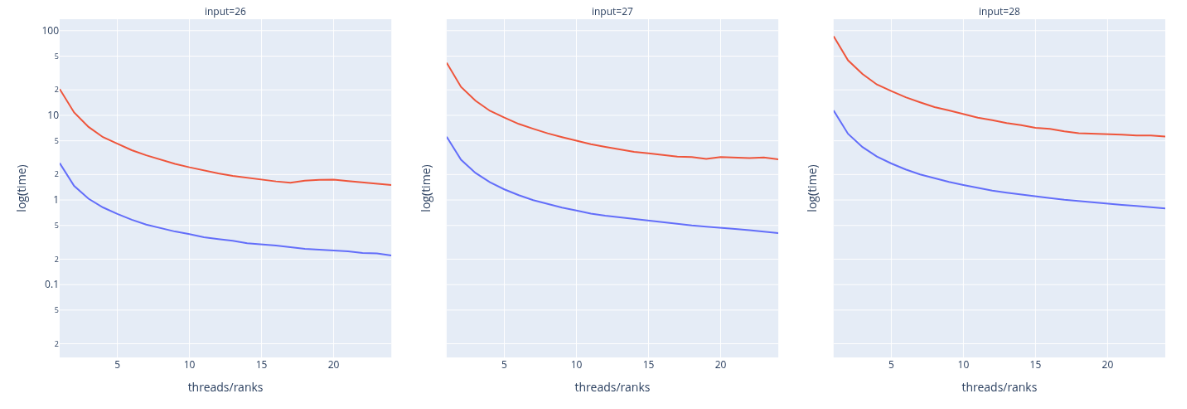
\includegraphics[scale=0.3]{fig_design/figure1.png}
\end{figure}

\item \textbf{Speedup \UPMEM vs Multicore}: the ratio of execution time for 1 thread on multicore divided by the execution time for 1 rank on \UPMEM.

\begin{figure}[H]
\centering
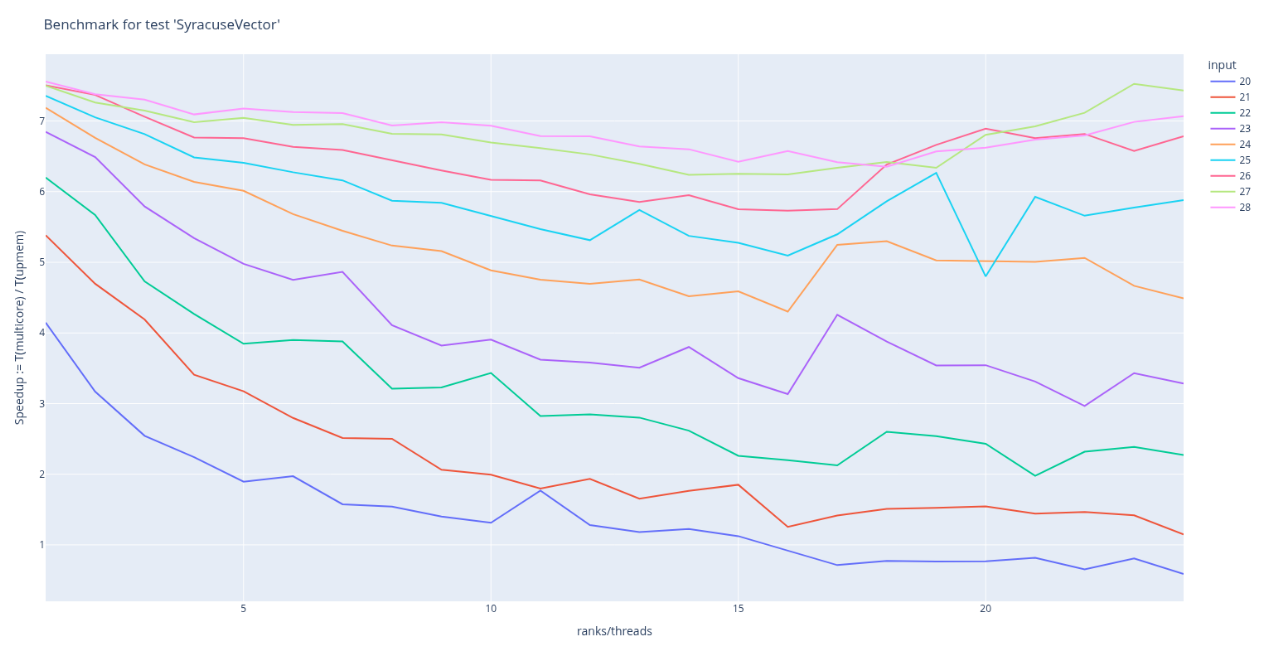
\includegraphics[scale=0.3]{fig_design/figure2.png}
\end{figure}

\item \textbf{Scalability per architecture}: for both multicore and \UPMEM, this section displays scalability per process unit. For a given number $N$ of process units (threads or ranks, ie. 16*64*tasklets per rank), the ratio of the execution time for 1 process unit to that for $N$ process units is shown.

\begin{figure}[H]
\centering
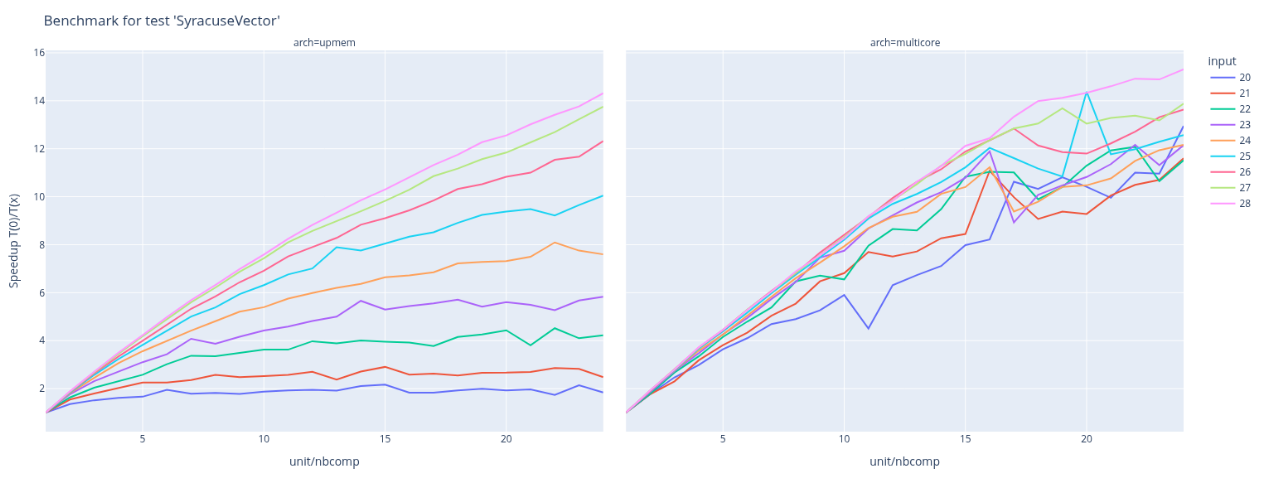
\includegraphics[scale=0.3]{fig_design/figure3.png}
\end{figure}

\item \textbf{Overheads for the \UPMEM architecture}: the \BPL provides statistics for overheads specific to \UPMEM. These timings are measured from the host's perspective, not the DPU's.

\begin{itemize}
\item \textbf{launch}: execution time of the task, i.e., the execution of the \cxx{dpu\_launch} function (with \cxx{DPU\_SYNCHRONOUS} argument).
\item \textbf{pre}: preparation and broadcasting of the input data from the host to the DPU (including call to scatter/gather function \cxx{dpu\_push\_sg\_xfer})
\item \textbf{post}: retrieval of output metadata from the DPU to the host (call to \cxx{dpu\_push\_xfer} function). This metadata is used to reconstruct the task result.
\item \textbf{result}: preparation and transmission of the task’s output data back to the host (calls to \cxx{dpu\_copy\_from\_mrams} for instance)
\item \textbf{unknown}: parts that cannot be measured in the previous categories (e.g., destructors) are included here.
\end{itemize}

In the following example, preparing and sending the input data to the DPU takes a significant amount of time compared to the actual processing.


\begin{figure}[H]
\centering
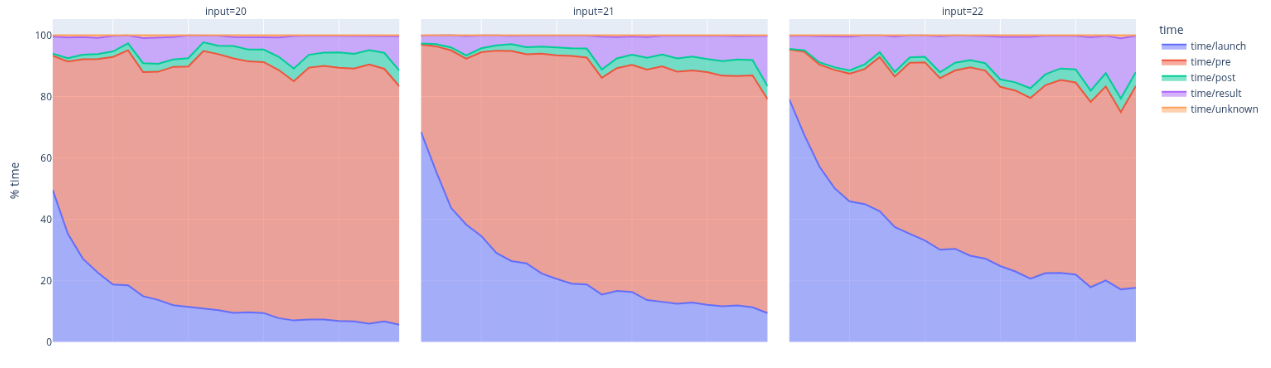
\includegraphics[scale=0.3]{fig_design/figure4.png}
\end{figure}
\end{itemize}

The execution times recorded during benchmarking are summarized in tables at the end of the report. While this may appear verbose, it can be very useful for referencing specific values from previous benchmark runs. Creating a benchmark test suite is not straightforward, as there is no clear rule for deciding when to add a test. A good rule of thumb is to be fair with respect to the library’s features: include tests where the library performs well on the \UPMEM architecture compared to multicore (e.g., small data / heavy computation), but also include cases where \UPMEM overheads are significant (e.g., large data / light computation).

For example, \cxx{SketchJaccardDistance} compares all possible pairs of sketches, resulting in a triple loop scanning the data. This is a scenario that favors \UPMEM because the broadcast cost is small compared to the total computation time. On the other hand, sorting a vector with an $O(n \log n)$ algorithm is likely faster on multicore, because on \UPMEM the broadcasts (host → DPU for input and DPU → host for output) can take a significant amount of time relative to the sorting itself. Therefore, it is important to select tests for benchmarking based on the computational complexity relative to the data size to be broadcast.

Another consideration is the total execution time of the benchmark suite. Since the same test is run with multiple input parameters, execution times can grow quickly. It is therefore important not to include too many tests, or the benchmark could take an excessively long time to complete.

Each new version of the BPL should commit the raw data generated during benchmark execution. This makes it possible to compare two versions and identify any improvements in execution time. A dedicated Jupyter notebook could be created to visualize the differences between the two versions using graphics.

\subsection{The LOC metric}

So far, we have tested the BPL through unit tests and benchmarks.
There is an additional way to evaluate the BPL, from the developer's perspective, in cases where one wants to use the UPMEM architecture: does the BPL allow for faster development compared to using the UPMEM SDK?

To ensure a fair comparison, we will assume here that the developer has equivalent knowledge of (1) the UPMEM SDK and (2) the BPL API; in other words, that they possess sufficient understanding of both APIs to write code directly using either approach.
\footnote{In practice, the learning curve for the UPMEM SDK remains more complex than that of the BPL.}

Therefore, the metric that comes to mind is the number of lines of code required to write a program, either using the UPMEM API or the BPL API.
From now on, this metric will be referred to as LOC, for "Lines Of Code."

Of course, it is not practical to write every program using both approaches in order to compare the LOC, since the goal is primarily to develop using the BPL API. However, it is still interesting to perform this exercise on a few examples.

In the following, we will assess the task of calculating the checksum of a buffer, as this is an example provided in the UPMEM documentation. We can therefore simply write the BPL version and compare the LOC in both cases.
Here is the UPMEM SDK version. First the DPU part (with all comments removed):

\begin{minted}[bgcolor=bg,linenos]{c++}
#include <mram.h>
#include <stdbool.h>
#include <stdint.h>
#define CACHE_SIZE 256
#define BUFFER_SIZE (1 << 16)
__mram_noinit uint8_t buffer[BUFFER_SIZE];
__host uint32_t checksum;
int main() {
  __dma_aligned uint8_t local_cache[CACHE_SIZE];
  checksum = 0;
  for (unsigned int bytes_read = 0; bytes_read < BUFFER_SIZE;) {
    mram_read(&buffer[bytes_read], local_cache, CACHE_SIZE);
    for (unsigned int byte_index = 0; (byte_index < CACHE_SIZE) 
         && (bytes_read < BUFFER_SIZE); byte_index++, bytes_read++) {
      checksum += (uint32_t)local_cache[byte_index];
    }
  }
  return checksum;
}
\end{minted}

and the host part


\begin{minted}[bgcolor=bg,linenos]{c++}
#include <dpu.h>
#include <assert.h>
#include <stdint.h>
#include <stdio.h>
#ifndef DPU_BINARY
#define DPU_BINARY "trivial_checksum_example"
#endif
#define BUFFER_SIZE (1 << 16)
void populate_mram(struct dpu_set_t set, uint32_t nr_dpus) {
  struct dpu_set_t dpu;
  uint32_t each_dpu;
  uint8_t *buffer = malloc(BUFFER_SIZE * nr_dpus);
  DPU_FOREACH(set, dpu, each_dpu) {
    for (int byte_index = 0; byte_index < BUFFER_SIZE; byte_index++) {
      buffer[each_dpu * BUFFER_SIZE + byte_index] = (uint8_t)byte_index;
    }
    buffer[each_dpu * BUFFER_SIZE] += each_dpu; 
    DPU_ASSERT(dpu_prepare_xfer(dpu, &buffer[each_dpu * BUFFER_SIZE]));
  }
  DPU_ASSERT(dpu_push_xfer(set, DPU_XFER_TO_DPU, "buffer", 0, BUFFER_SIZE, 
  	DPU_XFER_DEFAULT));
  free(buffer);
}
void print_checksums(struct dpu_set_t set, uint32_t nr_dpus) {
  struct dpu_set_t dpu;
  uint32_t each_dpu;
  uint32_t checksums[nr_dpus];
  DPU_FOREACH(set, dpu, each_dpu) {
    DPU_ASSERT(dpu_prepare_xfer(dpu, &checksums[each_dpu]));
  }
  DPU_ASSERT(dpu_push_xfer(set, DPU_XFER_FROM_DPU, "checksum", 0, 
  	sizeof(uint32_t), DPU_XFER_DEFAULT));
  DPU_FOREACH(set, dpu, each_dpu) {
    printf("[%u] checksum = 0x%08x\n", each_dpu, checksums[each_dpu]);
  }
}
int main() {
  struct dpu_set_t set, dpu;
  DPU_ASSERT(dpu_alloc(DPU_ALLOCATE_ALL, NULL, &set));
  DPU_ASSERT(dpu_load(set, DPU_BINARY, NULL));
  DPU_ASSERT(dpu_get_nr_dpus(set, &nr_dpus));
  populate_mram(set, nr_dpus);
  DPU_ASSERT(dpu_launch(set, DPU_SYNCHRONOUS));
  print_checksums(set, nr_dpus);
  DPU_ASSERT(dpu_free(set));
  return 0;
}
}\end{minted}

which totals $19+47$ lines, or $66$ in all.

Now, using the BPL API, we have:

\begin{minted}[bgcolor=bg,linenos]{c++}
#include <bpl/core/Task.hpp>
template<class ARCH>
struct VectorChecksum : bpl::Task<ARCH>  {
    USING(ARCH);
    auto operator() (vector<uint32_t> const& v)  {
        return accumulate(v.begin(), v.end(), uint64_t{0});
    }
    static uint64_t reduce (uint64_t a, uint64_t b)  { return a+b; }
};
\end{minted}

and

\begin{minted}[bgcolor=bg,linenos]{c++}
#include <vector>
#include <cstdio>
#include <bpl/bpl.hpp>
int main() {
    std::vector<uint32_t> v;  
    for (size_t i=1; i<=1<<16; i++)  {  v.push_back(i);  }
    Launcher<ArchUpmem> launcher {1_dpu};
    printf ("checksum: %ld\n", launcher.run<VectorChecksum>(split(v)));
}
}\end{minted}

which totals $9+9$ lines, or $18$ in all. 

Thus, we have 66 LOC for the UPMEM SDK and 18 LOC for the BPL, a ratio of 3.66. Note that the ratio would be 3.88 if we count characters instead of lines.

In addition to the significant reduction in code size with the BPL, code written using the BPL is also much more readable than with the UPMEM SDK. Indeed, reading the BPL code makes it immediately clear that the task is to compute the checksum of a vector, which is far less obvious in the UPMEM SDK version, 
where all the low-level SDK calls reduce overall readability.

Of course, it would be worthwhile to extend this LOC comparison to other examples, but it seems fairly clear that the advantage would still favor the BPL.
The remaining point to determine is the overhead of the BPL compared to writing directly using the UPMEM SDK.  If a BPL version were consistently 50\% slower than a SDK version, its usefulness could be limited. In this regard, benchmark tests can provide a typology of algorithms that are likely to benefit from execution via the BPL on a UPMEM architecture, and conversely, those that might be penalized.

Related to readability, it is also conceivable that a developer could implement a simple algorithm using the BPL to run on a UPMEM architecture  without needing to know the UPMEM SDK, which would represent a significant benefit of the BPL.


\section{Workloads}

\subsection{Bloom filters library for large batches of items}
\label{sec:bfs}

\paragraph{Presentation}
BFlib is a Bloom filters library aimed at storing and querying large chunks of elements at once.
Instead of one big array, the library uses a collection of smaller filters.
The library is specifically designed to run with the Processing-in-Memory hardware from UPMEM, in which case the many filters actually reside on different memory banks.
Efficient parallel processing can thus be performed to execute large batches of insertions or lookups.
We re-implement this processing using the BPL library.

\paragraph{Limitations encountered} Since we execute insertions and lookups in batches, the filters need to exist in memory across several executions.
However, the BPL does not support such feature at the moment.
Therefore, we had to design an additional class to manage persistent storage and implement it for all architectures supported by the BPL.
For UPMEM, the persistent data block is reserved in the MRAM of each DPU.
As for Multicore, we allocate all data blocks required, store them in a vector, and adds an index argument to the task so that each instance can retrieve its assigned block.

\paragraph{Benchmarks} We consider Bloom filters using 8 hash functions, and a varying size (128 KiB or 1 MiB).
For PiM implementations, we allocate 8 ranks, i.e. 512 processing units.
One benchmark consists of inserting a varying number of items (10M or 100M), and then querying all the inserted items.

\begin{table}[htbp]
    \centering
    \caption{Results of the Bloom filters benchmarks}
    \label{tab:bflib-results}
    \begin{tabular}{lrrrrrr}
    \toprule
     & & & \multicolumn{2}{c}{Multicore time (s)} & \multicolumn{2}{c}{PiM time (s)} \\
    \cmidrule(l{3pt}r{3pt}){4-5}\cmidrule(l{3pt}r{3pt}){6-7}
    & Filter size & \#items & Standard* & BPL & SDK & BPL \\
    \midrule
    \multirow{4}{*}{Insertions} & 128 MiB & 10M & 0.22 & 0.56 & 0.13 & 0.11 \\
    & 128 MiB & 100M & 1.49 & 4.64 & 0.66 & 0.68 \\
    & 1 GiB & 10M & 0.39 & 0.84 & 0.13 & 0.11 \\
    & 1 GiB & 100M & 2.24 & 5.56 & 0.66 & 0.68 \\
    \midrule
    \multirow{4}{*}{Lookups} & 128 MiB & 10M & 0.25 & 0.41 & 0.27 & 0.28 \\
    & 128 MiB & 100M & 2.26 & 3.06 & 2.13 & 2.26 \\
    & 1 GiB & 10M & 0.38 & 0.38 & 0.27 & 0.28 \\
    & 1 GiB & 100M & 2.89 & 2.94 & 2.13 & 2.81 \\
    \bottomrule
    \end{tabular}
    \\ \vspace{0.3em}
    {\scriptsize *Uses a single big filter and not the many small filters approach}
\end{table}

\paragraph{Results} We present the results in \tablename~\ref{tab:bflib-results}.
The Standard Multicore implementation appears faster than the BPL Multicore version, due to being less memory-bound.
Indeed, it handles items one at a time instead of regrouping them in batches and processing them altogether.
Batching is beneficial with the PiM architecture to minimize the overhead of transferring data between the main memory and the small memory banks, but this purpose is absent on Multicore.
Implementing a program on several architectures at once is a great perk of the BPL, but this comes with a caveat: it forces to use the same parallelization scheme for both Multicore and PiM, which is not necessarily the best choice performance-wise.
Regarding PiM, the BPL version has similar execution times to the SDK program.

\paragraph{Source code} The BPL implementation is publicly available at \url{https://gitlab.inria.fr/pim/org.pim.bflib-bpl} (GNU AGPLv3).
The original Standard Multicore and SDK implementations are available at \url{https://gitlab.inria.fr/pim/org.pim.bloomfilters} (GNU AGPLv3).

\subsection{Mapping based on Hamming distance}
\label{sec:mapping}

\paragraph{Presentation}MiMyCS is a software that performs reference-based lossless compression of next-gen sequencing datasets~\cite{DeMoor2024}.
It relies on mapping each read against a known reference and storing the mapping position along with potential substitution errors.
The mapping stage is implemented with PiM acceleration by partitioning the reference across memory banks and sending reads to map to only a few well-chosen processing units.
We re-implement this mapping procedure using the BPL library.

\paragraph{Limitations encountered} We process the reference and need to store the resulting indexing information for all future mapping executions.
However, the BPL does not support such feature at the moment.
Therefore, we had to design an additional class to manage persistent storage and implement it for all architectures supported by the BPL.
For UPMEM, the persistent indexing tables are allocated in the MRAM of each DPU.
As for Multicore, we allocate all tables required, store them in a vector, and adds an index argument to the task so that each instance can retrieve its assigned tables.

\paragraph{PiM specifics} To perform the Hamming distance computations as efficiently as possible on the UPMEM architecture, we write manually a few lines of assembly instructions.
This part of the task thus uses target-specific code.

\paragraph{Benchmarks} We consider a real whole genome sequencing dataset obtained with the Illumina technology, known as accession code SRR14724532 on the European Nucleotide Archive portal.
We map this dataset against the human genome GRCh38.
For PiM, we use 8 ranks as this is the minimum required to fit the entire reference genome across all memory banks.
We report the execution time of the two stages: indexing the reference, and mapping all the reads of the dataset.

\begin{table}[htbp]
    \centering
    \caption{Results of the mapping benchmark}
    \label{tab:mapping-results}
    \begin{tabular}{lrrrr}
    \toprule
     &\multicolumn{2}{c}{Multicore time (s)} & \multicolumn{2}{c}{PiM time (s)} \\
    \cmidrule(l{3pt}r{3pt}){2-3}\cmidrule(l{3pt}r{3pt}){4-5}
    & Standard & BPL & SDK & BPL \\
    \midrule
    Indexing reference & 33.1 & 49.4 & 20.4 & 34.2 \\
    Mapping reads & 104.6 & 142.2 & 59.1 & 92.8 \\
    \bottomrule
    \end{tabular}
\end{table}

\paragraph{Results} We present results in \tablename~\ref{tab:mapping-results}.
For both the indexing and the mapping, we see that the BPL introduces a non-negligible overhead and is 63\% slower compared to the optimized SDK version.
The overhead is for the most part due to the serialization process when retrieving the task results back to the host.
Indeed, this involves several memory copies: first on the DPUs, to re-aggregate all the tasklets results into a single buffer, and then on the host, to reformat the transferred buffer into the expected type.
All of these copies do not exist when using the SDK.

\paragraph{Source code} The BPL implementation is publicly available at \url{https://gitlab.inria.fr/pim/org.pim.mimycs-bpl} (GNU AGPLv3).
The original Standard Multicore and SDK implementations are available at \url{https://gitlab.inria.fr/pim/org.pim.srm} (GNU AGPLv3).

\subsection{Primer alignment with the Smith-Waterman algorithm}
\label{sec:conclud}

\paragraph{Presentation}ConCluD is a software that relies on De-Buijn graph partitioning to generate consensus sequences in the context of DNA storage decoding~\cite{DeMoor2025}.
The partitioning step requires to align reads against a set of known primers to find the best fitting one.
The published version of ConCluD uses a simple approach based on the Hamming distance.
Such computation has already been investigated in Section~\ref{sec:mapping} with the MiMyCS software.
To explore a different scenario, we thus decide to rather re-implement with the BPL library an older version of ConCluD where the alignment step was originally done with the Smith-Waterman algorithm.

\paragraph{Limitations encountered} None: the code can be fully architecture-agnostic.

\paragraph{PiM specifics} To perform the alignment computations as efficiently as possible on the UPMEM architecture, we write manually a few lines of assembly code.
In particular, we take advantage of the \texttt{cmp4} instruction to compare four bytes at once.
This part of the task thus uses target-specific code.

\paragraph{Benchmarks} We use three real datasets from the experimental evaluation in ~\cite{DeMoor2025}, namely Odeuropa, Dunhuang-d0 and HorrorMovie.
For PiM, we use 32 ranks.

\paragraph{Results} We give results in \tablename~\ref{tab:sw-results}.
On all datasets, the BPL version is slower than the SDK version regarding the PiM architecture.
For the largest dataset, HorrorMovie, it is 34\% slower.
On top of the BPL overhead, another reason contributes to this observation: we had to split the work statically between tasklets to keep the program entirely architecture-agnostic with regard to the current BPL features.
On the other hand, the SDK version uses dynamic scheduling to assign reads to tasklets on the same DPU.
The latter is more efficient because the processing time of a read can differ drastically: some reads lead to a perfect alignment very fast, while other require to go through the whole Smith-Waterman matrix or even try several primers.

Regarding the Multicore target, the BPL version is also slower, except for the Dunhuang-d0 dataset where it is faster.
The fact that the BPL version processes reads in batches instead of one at a time, combined with the dataset having only one primer, seem to make the BPL version less memory-bound that the Standard program in this case.

\begin{table}[htbp]
    \centering
    \caption{Results of the primer alignment benchmark}
    \label{tab:sw-results}
    \begin{tabular}{lrrrr}
    \toprule
    & \multicolumn{2}{c}{Multicore time (s)} & \multicolumn{2}{c}{PiM time (s)} \\
    \cmidrule(l{3pt}r{3pt}){2-3}\cmidrule(l{3pt}r{3pt}){4-5}
    & Standard & BPL & SDK & BPL \\
    \midrule
    Odeuropa & 12.5 & 16.3 & 4.7 & 6.7 \\
    Dunhuang-d0 & 37.0 & 25.8 & 12.4 & 20.6 \\
    HorrorMovie & 262.4 & 382.0 & 92.3 & 123.9 \\
    \bottomrule
    \end{tabular}
\end{table}

\paragraph{Source code} The BPL implementation is publicly available at \url{https://gitlab.inria.fr/pim/org.pim.conclud-bpl} (GNU AGPLv3).
The original Standard Multicore and SDK implementations are available at \url{https://gitlab.inria.fr/pim/org.pim.dnarxiv/-/tags/experiments-bioRxiv-preprint} (GNU AGPLv3).

\subsection{Sort}
\label{sec:sort}

\paragraph{Presentation}
Sort workloads consist of a series of independent applications of small sorting algorithms.
In this implementation, the size of the data to be sorted is fixed, as the primary objective is benchmarking against CPU and BPL implementations.
Each application sorts a large number of independent arrays.

\paragraph{Limitations encountered}
The BPL code executed on CPU and PiM is identical; however, the application was originally designed to run on PiM.
As a result, the applications are constrained by the maximum array size that can be sorted.

\paragraph{PiM specifics}
In addition to the BPL version, SDK-based implementations are also provided, as for other workloads.
No special instructions are used.
The SDK versions are available in two variants: one relying on an automatic cache between MRAM and WRAM (SDK-C), implemented in this work using an RRIP-based policy, and another using explicit manual data transfers(SDK).

\paragraph{Benchmarks}
Uniformly distributed random arrays of \texttt{int32} values are used as input.
The number of arrays being sorted depends on the number of ranks (real or emulated), scaling up to 40{,}960.
The array size is limited by the MRAM capacity and the MRAM memory overhead introduced by BPL, and all benchmarks are conducted using the maximum supported size of 131{,}072 elements.
Each benchmark is executed five times, and the reported results correspond to the mean value.
To give CPU implementations the best possible performance, applications are compiled with the flags \texttt{-march=native} and \texttt{-O3}.
Additionally, an Intel-optimized version of Quicksort is included (indicated in parentheses).



\paragraph{Results}

\begin{table}[!t]
\centering
{\footnotesize
\renewcommand{\arraystretch}{0.85}
\setlength{\aboverulesep}{1pt}
\setlength{\belowrulesep}{2pt}
\setlength{\cmidrulewidth}{0.1pt}
\setlength{\cmidrulekern}{0pt}

\caption{Aggregated results of sorting benchmark across all ranks and array sizes}
\label{tab:sort-results-all}

\begin{tabular}{lllrrrrr}
\toprule
& & & \multicolumn{2}{c}{Multicore time (s)} & \multicolumn{3}{c}{PiM time (s)} \\
\cmidrule(l{3pt}r{3pt}){4-5}\cmidrule(l{3pt}r{3pt}){6-8}
Rank & ARR\_SIZE & Algorithm & Standard & BPL & SDK & SDK-C & BPL \\
\midrule
    \multirow{9}{*}{1} & \multirow{3}{*}{131072} & Quicksort & 0.5 (0.1) & 0.5 & 4.9 & 5.9 & 8.2 \\
     &  & Heapsort  & 0.7 & 0.7 & 25.4 & 19.9 & 25.0 \\
     &  & Radixsort & 0.2 & 0.2 & 3.2 & 4.3 & 6.4 \\
\cmidrule(l{3pt}r{3pt}){2-8}
     & \multirow{3}{*}{262144} & Quicksort & 1.0 (0.2) & 1.0 & 10.1 & 12.7 & 17.6 \\
     &  & Heapsort  & 1.6 & 1.6 & 54.1 & 42.3 & 52.1 \\
     &  & Radixsort & 0.5 & 0.7 & 6.5 & 8.3 & NA \\
\cmidrule(l{3pt}r{3pt}){2-8}
     & \multirow{3}{*}{524288} & Quicksort & 2.1 (0.6) & 2.1 & 21.3 & 26.8 & NA \\
     &  & Heapsort  & 3.3 & 4.3 & 115.0 & 89.4 & NA \\
     &  & Radixsort & 1.4 & 1.5 & 13.0 & 16.5 & NA \\
\midrule 
    \multirow{9}{*}{10} & \multirow{3}{*}{131072} & Quicksort & 4.8 (1.0) & 4.7 & 6.5 & 7.4 & 12.3 \\
     &  & Heapsort  & 7.0 & 6.9 & 26.9 & 21.4 & 28.4 \\
     &  & Radixsort & 1.5 & 1.8 & 4.8 & 5.7 & 10.2 \\
\cmidrule(l{3pt}r{3pt}){2-8}
     & \multirow{3}{*}{262144} & Quicksort & 10.1 (2.5) & 9.8 & 13.2 & 15.5 & 24.8 \\
     &  & Heapsort  & 15.9 & 15.1 & 57.2 & 45.4 & 59.4 \\
     &  & Radixsort & 6.2 & 5.9 & 9.6 & 11.2 & NA \\
\cmidrule(l{3pt}r{3pt}){2-8}
     & \multirow{3}{*}{524288} & Quicksort & 21.0 (6.8) & 20.3 & 27.5 & 32.9 & NA \\
     &  & Heapsort  & 48.0 & 42.4 & 121.5 & 95.4 & NA \\
     &  & Radixsort & 14.7 & 13.8 & 19.0 & 22.6 & NA \\
\midrule
    \multirow{9}{*}{20} & \multirow{3}{*}{131072} & Quicksort & 9.6 (1.8) & 9.4 & 7.2 & 8.2 & 14.4 \\
     &  & Heapsort  & 13.9 & 13.8 & 27.7 & 22.2 & 30.3 \\
     &  & Radixsort & 2.9 & 3.4 & 5.6 & 6.5 & 12.4 \\
\cmidrule(l{3pt}r{3pt}){2-8}
     & \multirow{3}{*}{262144} & Quicksort & 20.2 (4.9) & 19.6 & 14.4 & 16.8 & 29.0 \\
     &  & Heapsort  & 31.8 & 30.1 & 58.6 & 46.6 & 63.7 \\
     &  & Radixsort & 11.9 & 11.5 & 10.8 & 12.5 & NA \\
\cmidrule(l{3pt}r{3pt}){2-8}
     & \multirow{3}{*}{524288} & Quicksort & 41.9 (13.2) & 40.5 & 29.2 & 34.5 & NA \\
     &  & Heapsort  & 95.4 & 85.5 & 123.5 & 97.3 & NA \\
     &  & Radixsort & 29.3 & 27.7 & 20.8 & 24.5 & NA \\
\midrule
    \multirow{9}{*}{30} & \multirow{3}{*}{131072} & Quicksort & 14.4 (2.8) & 14.0 & 8.2 & 9.1 & 16.8 \\
     &  & Heapsort  & 20.8 & 20.6 & 28.5 & 22.9 & 32.8 \\
     &  & Radixsort & 4.4 & 5.1 & 6.5 & 7.3 & 14.6 \\
\cmidrule(l{3pt}r{3pt}){2-8}
     & \multirow{3}{*}{262144} & Quicksort & 30.2 (7.2) & 29.3 & 15.8 & 18.2 & 34.3 \\
     &  & Heapsort  & 46.9 & 45.0 & 59.8 & 47.8 & 68.3 \\
     &  & Radixsort & 17.7 & 17.1 & 12.2 & 14.0 & NA \\
\cmidrule(l{3pt}r{3pt}){2-8}
     & \multirow{3}{*}{524288} & Quicksort & 62.0 (19.9) & 60.6 & 31.7 & 37.2 & NA \\
     &  & Heapsort  & 102.7 & 126.6 & 126.0 & 99.9 & NA \\
     &  & Radixsort & 43.9 & 40.7 & 23.8 & 27.2 & NA \\
\midrule
    \multirow{9}{*}{40} & \multirow{3}{*}{131072} & Quicksort & 19.2 (3.7) & 18.7 & 8.8 & 9.9 & 19.3 \\
     &  & Heapsort  & 27.8 & 27.5 & 29.2 & 23.7 & 35.0 \\
     &  & Radixsort & 5.9 & 7.0 & 7.2 & 8.1 & 17.0 \\
\cmidrule(l{3pt}r{3pt}){2-8}
     & \multirow{3}{*}{262144} & Quicksort & 40.3 (9.5) & 39.0 & 17.3 & 19.8 & 38.3 \\
     &  & Heapsort  & 63.5 & 60.0 & 61.1 & 49.0 & 73.1 \\
     &  & Radixsort & 23.9 & 22.9 & 13.7 & 15.5 & NA \\
\cmidrule(l{3pt}r{3pt}){2-8}
     & \multirow{3}{*}{524288} & Quicksort & 82.6 (26.2) & 80.8 & 34.5 & 40.3 & NA \\
     &  & Heapsort  & 136.8 & 167.9 & 128.4 & 102.8 & NA \\
     &  & Radixsort & 58.2 & 55.4 & 26.6 & 29.7 & NA \\
\bottomrule
\end{tabular}}
\end{table}

We report the results of the sorting benchmark in Table~\ref{tab:sort-results-all}.
On both targets, the BPL implementation is consistently slower than the architecture-specific versions.
On the PiM architecture, the BPL version exhibits a significant overhead compared to the SDK and SDK-C implementations for all sorting algorithms.
For instance, in the case of Quicksort, the BPL version is almost four times slower than the SDK version.
This overhead will be further analyzed once execution traces are available.

On the Multicore target, similar trends are observed.
The BPL version remains slower than the Standard implementation for all algorithms.
The current implementation suffers from unnecessary memory copies, even though the data are already accessible to the CPU cores.
Overall, these results highlight the performance cost of maintaining portability and architecture-agnosticism with BPL.

\subsection{Sketches comparison}
\label{sec:mash}

\paragraph{Presentation}

We present here a benchmark comparing sketches.
As a reminder,, 
Comparing two genomic sequences can therefore be approximated by comparing two sketches, that is, two ordered sequences of integers of the same size $N$,
which can be performed with a complexity of $O(N)$. 
As a result, a comparison score is produced, making it possible to estimate the similarity between the two genomic sequences.

\paragraph{Limitations encountered} 
For simplicity, the PIM version using the UPMEM SDK only allows certain sizes of the reference and query databases to be used.

\paragraph{Benchmarks} 
For this benchmark, we consider two databases: a reference database containing $R$ sketches, and a query database containing $Q$ sketches. The benchmark consists of performing the $R \cdot Q$ comparisons for each (ref, qry) pair. 
We will use sketches of $10,000$ integers, each integer encoded on $4$ bytes.

We choose to vary the sizes $R$ and $Q$ of the reference and query databases, as well as the number of compute units (threads for multicore and ranks for PIM).
In its largest configuration, the reference database contains 245,760 sketches of 10,000 integers of 4 bytes each, totaling over 9 GB of data.
For each configuration (reference database size, query database size), the list of scores is computed. A checksum of these scores is then calculated, and we verify that each implementation returns the same checksum for a given configuration, regardless of the number of compute units used.

\begin{table}
\caption{Results of the sketches comparison benchmark}
\label{tab:mash-results}
\begin{tabular}{lll|rr|rr}
\toprule
 &  &  & \multicolumn{4}{r}{duration} \\
 &  & type & 1.MC std & 2.MC BPL & 3.PIM SDK & 4.PIM BPL \\
ref & qry & nbunits &  &  &  &  \\
\midrule
\multirow[t]{8}{*}{\textbf{24576}} & \multirow[t]{4}{*}{\textbf{16}} & \textbf{3} & 1.79 & 2.11 & 1.31 & 1.07 \\
\textbf{} & \textbf{} & \textbf{6} & 0.93 & 1.10 & 0.71 & 0.59 \\
\textbf{} & \textbf{} & \textbf{12} & 0.48 & 0.57 & 0.41 & 0.37 \\
\textbf{} & \textbf{} & \textbf{24} & 0.34 & 0.38 & 0.26 & 0.24 \\
\cline{2-7}
\textbf{} & \multirow[t]{4}{*}{\textbf{128}} & \textbf{3} & 13.50 & 16.14 & 9.61 & 7.64 \\
\textbf{} & \textbf{} & \textbf{6} & 7.07 & 8.49 & 4.88 & 3.93 \\
\textbf{} & \textbf{} & \textbf{12} & 3.66 & 4.37 & 2.53 & 2.10 \\
\textbf{} & \textbf{} & \textbf{24} & 2.33 & 2.63 & 1.39 & 1.19 \\
\cline{1-7} \cline{2-7}
\multirow[t]{8}{*}{\textbf{122880}} & \multirow[t]{4}{*}{\textbf{16}} & \textbf{3} & 8.53 & 10.40 & 6.71 & 5.38 \\
\textbf{} & \textbf{} & \textbf{6} & 4.50 & 5.73 & 3.44 & 2.82 \\
\textbf{} & \textbf{} & \textbf{12} & 2.32 & 2.77 & 1.88 & 1.57 \\
\textbf{} & \textbf{} & \textbf{24} & 1.56 & 1.75 & 1.11 & 0.95 \\
\cline{2-7}
\textbf{} & \multirow[t]{4}{*}{\textbf{128}} & \textbf{3} & 67.22 & 80.53 & 47.83 & 37.97 \\
\textbf{} & \textbf{} & \textbf{6} & 35.42 & 42.27 & 24.15 & 19.26 \\
\textbf{} & \textbf{} & \textbf{12} & 18.35 & 21.88 & 12.29 & 9.84 \\
\textbf{} & \textbf{} & \textbf{24} & 9.71 & 11.66 & 6.41 & 5.11 \\
\cline{1-7} \cline{2-7}
\multirow[t]{8}{*}{\textbf{245760}} & \multirow[t]{4}{*}{\textbf{16}} & \textbf{3} & 17.79 & 20.77 & 13.70 & 10.89 \\
\textbf{} & \textbf{} & \textbf{6} & 9.33 & 11.09 & 6.88 & 5.68 \\
\textbf{} & \textbf{} & \textbf{12} & 4.64 & 5.79 & 3.92 & 3.23 \\
\textbf{} & \textbf{} & \textbf{24} & 2.81 & 3.42 & 2.21 & 1.87 \\
\cline{2-7}
\textbf{} & \multirow[t]{4}{*}{\textbf{128}} & \textbf{3} & 134.47 & 161.01 & 95.88 & 76.03 \\
\textbf{} & \textbf{} & \textbf{6} & 70.83 & 84.50 & 48.19 & 38.42 \\
\textbf{} & \textbf{} & \textbf{12} & 36.70 & 43.73 & 24.56 & 19.55 \\
\textbf{} & \textbf{} & \textbf{24} & 19.28 & 22.73 & 12.63 & 10.06 \\
\cline{1-7} \cline{2-7}
\bottomrule
\end{tabular}
\end{table}


\paragraph{Results} We present the results in \tablename~\ref{tab:mash-results}. The four implementations tested are:
\begin{enumerate}
\item \textbf{MC std}: the multicore implementation using standard threads; The {BS::thread\_pool} library is used to simplify thread management
\item \textbf{MC BPL}: the multicore implementation using the BPL
\item \textbf{PIM SDK}: an implementation directly using the UPMEM SDK; The reading of the reference and query databases is optimized using a local cache to minimize WRAM/MRAM transfers.
\item \textbf{PIM BPL}: the PIM implementation using the BPL
\end{enumerate}

As usual, there is actually a single BPL implementation, executed on both a multicore architecture and a PIM architecture. 
For this implementation, the reference database is partitioned into $K$ parts, with each thread or tasklet handling its own partition. The sketches from the query database are thus compared to each of these partitions.

For both PIM versions (SDK UPMEM and BPL) and for a fair comparison, it should be noted that the measured time does not include the duration of DPU allocation/deallocation.

Regarding the two multicore versions, we observe that the BPL version is slightly slower than the standard version, regardless of the configuration. This difference can be explained by two reasons. First, the data partitioning may be more advantageous for the standard version than for the multicore version, resulting in fewer cache misses and therefore fewer memory reloads. Second, the generic nature of the BPL version involves certain design and implementation choices that can sometimes prove less efficient than a more direct implementation.

For the two PIM versions, we observe slightly better performance for the BPL version. This result may seem counterintuitive, since the SDK version is conceptually close to what the BPL can produce in this example, notably with the same data partitioning. The compilation options for both versions are also equivalent for generating the DPU binaries. One possible explanation is that the compiler may be able to better optimize the BPL version compared to the SDK version.

We also observe that scalability is relatively good for all four versions. Since the number of compute units (i.e. threads or ranks) is doubled for each configuration, the execution time should in principle be halved, which is roughly what we observe. For example, none of the versions shows performance stagnation when the number of compute units is doubled.

Finally, for an equivalent number of threads and ranks, we observe that the PIM version is approximately twice as fast as the multithreaded version, whether comparing the two SDK versions or the two PIM versions.

\paragraph{Source code} The BPL implementation is publicly available at \url{https://gitlab.inria.fr/pim/org.pim.bpl/-/tree/main/test/xp/mash} (GNU AGPLv3)


\subsection{Sequences comparison}
\label{sec:pang}

\paragraph{Presentation}

Sequence comparison is an essential task in genomics, for example to search whether an unknown sequence can be found in a reference database. For instance, the software BLAST has enabled such comparisons for several decades now. Due to the considerable increase in the volume of available sequences, many successors have attempted to improve the underlying algorithm and/or take advantage of the parallelization capabilities of hardware architectures. 

We propose here to implement a version of the BLAST algorithm with no gap for the comparison of amino acid sequences on a PIM-type architecture. This version will be called PANG (Protein Alignment with No Gap) and the equivalent command line for the original BLAST would be

\begin{minted}[bgcolor=bg]{bash}
blastp -query <query.fasta> -subject <db.fasta> -ungapped -out <output> 
   -comp_based_stats F -evalue <evalue> -seg yes 
\end{minted}


\paragraph{Limitations encountered}
None: the BPL code can be fully architecture-agnostic.


\paragraph{Benchmarks} 

In the following, we will compare a PIM/SDK version of the PANG algorithm with a version implemented using BPL. Note that some heuristics differ slightly, so we will also examine the results themselves in addition to the performance aspects. 

We perform a comparison between the well-known SwissProt protein database and a subset of proteins from Arabidopsis thaliana. These two databases contain 563,082 and 15,873 proteins respectively, corresponding to a total of 202,799,066 and 6,788,821 amino acids. 
For both implementations, we used several different parameter settings, with E-values of 1e-3, 1e-6 and 1e-18 respectively.
For the SDK/UPMEM and BPL/UPMEM versions, one rank was used, corresponding to 64 DPUs.

\paragraph{Results}

We present the results in \tablename~\ref{tab:pang-results} that compares SDK and BPL implementation for an UPMEM architecture. 

\begin{table}[htbp]
    \centering
    \caption{Execution times for Arabidopsis thaliana vs. Swissprot}
    \label{tab:pang-results}
    \begin{tabular}{lrr}
    \toprule
    & PIM/SDK & PIM/BPL \\
    \midrule
    evalue=1e-3 & 1892 & 1615  \\
    \midrule
    evalue=1e-6 & 1785 & 1564  \\
    \midrule
    evalue=1e-18 & 1781 & 1523  \\
    \bottomrule
    \end{tabular}
\end{table}

The BPL version exhibits slightly better performance than the version implemented directly with the UPMEM SDK, 
which may be due to the slightly different heuristics used in the two implementations. 
To better assess this aspect, the Venn diagrams in figure [\ref{fig:pang-venn}]  illustrate the overlap between the [refId, qryId] pairs produced 
by the two versions. Most of the results are common to both versions, with some results specific to each implementation, likely as a consequence of the different heuristics employed. It can also be observed that for increasingly smaller evalues, the share specific to the BPL version decreases, so that the results obtained by the BPL version are almost included in the results obtained by the SDK version.
The fact that the SDK version produces more results may partly explain its slightly longer execution time.

\begin{figure}
    \centering
    \begin{minipage}{0.32\textwidth}
        \centering
        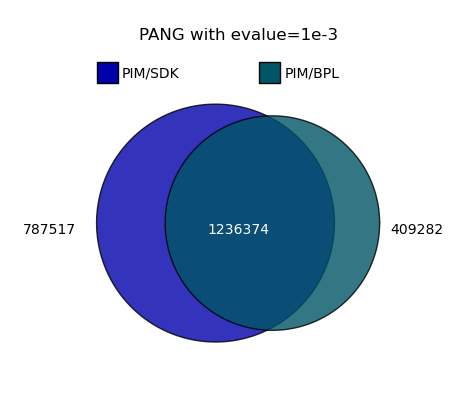
\includegraphics[width=1.1\textwidth]{fig_misc/pang.resulte3.png} % first figure itself
    \end{minipage}\hfill
    \begin{minipage}{0.32\textwidth}
        \centering
        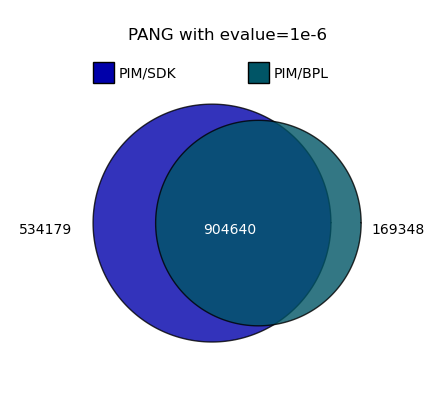
\includegraphics[width=1.1\textwidth]{fig_misc/pang.resulte6.png} % second figure itself
    \end{minipage}
    \begin{minipage}{0.32\textwidth}
        \centering
        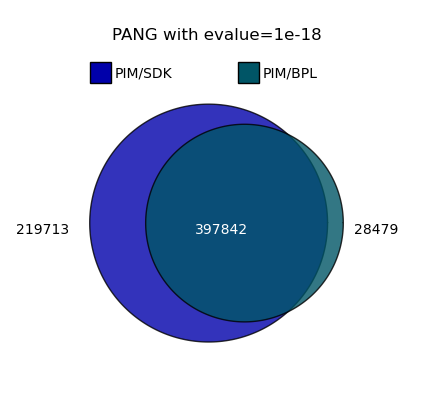
\includegraphics[width=1.1\textwidth]{fig_misc/pang.resulte18.png} % second figure itself
    \end{minipage}
	\caption{Comparing PANG results}
	\label{fig:pang-venn}
\end{figure}

In conclusion, we present several remarks regarding the scalability of the BPL version on multicore and UPMEM architectures. Figure [\ref{fig:pang-scalability}] (left) shows scalability as a function of the number of threads (for multicore) and the number of ranks (for UPMEM). The UPMEM version exhibits good scalability, remaining close to linear, whereas the multicore version shows a noticeable degradation as the number of threads increases. On the right, we analyze the speedup between the multicore and UPMEM versions for an equivalent number of threads/ranks. It can be observed that the UPMEM version benefits from increasing resources, showing improved performance.

\begin{figure}
    \centering
    \begin{minipage}{0.5\textwidth}
        \centering
        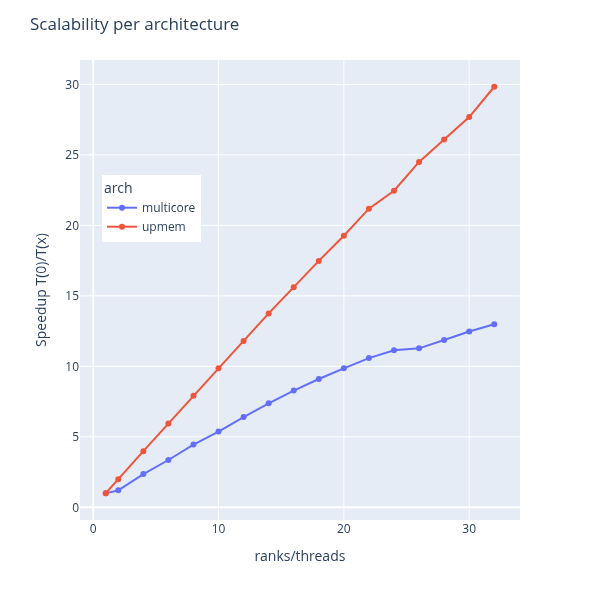
\includegraphics[width=1.0\textwidth]{fig_misc/pang_scalability.png} % first figure itself
    \end{minipage}\hfill
    \begin{minipage}{0.5\textwidth}
        \centering
        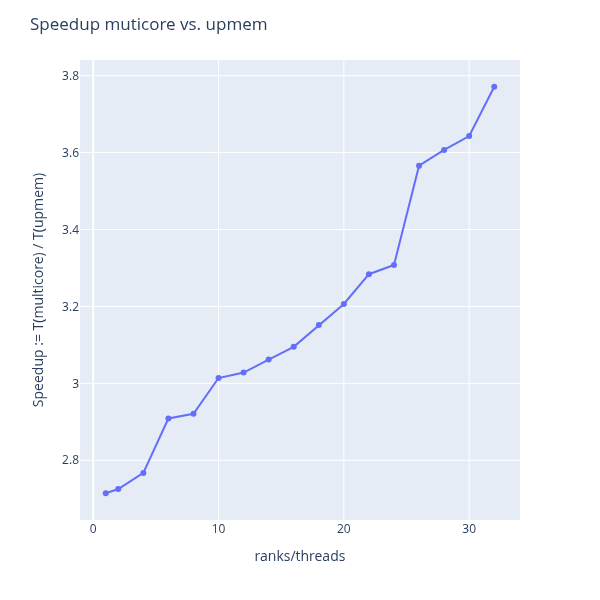
\includegraphics[width=1.0\textwidth]{fig_misc/pang_compare_arch.png} % second figure itself
    \end{minipage}
	\caption{PANG scalability for BPL versions}
	\label{fig:pang-scalability}
\end{figure}

\paragraph{Source code} The BPL implementation is publicly available at \url{https://gitlab.inria.fr/pim/org.pim.pang}.
The UPMEM SDK implementation is publicly available at \url{https://gitlab.inria.fr/pim/pang-sdk}.


\subsection{Pattern matching}
\label{sec:pmatch}

\paragraph{Presentation}

Searching for a pattern within a text is a common operation in various fields of applications, for instance for natural language processing, but also in genomics with a reduced alphabet containing the four DNA nucleotides.
We consider three state-of-the-art pattern matching algorithms: Aho-Corasick (AC), Knuth-Morris-Pratt (KMP) and Boyer-Moore (BM).
The Aho-Corasick algorithm~\cite{Aho1975} allows to search for multiple patterns while scanning the text only once, by representing the patterns in a trie and adding failure links to create an automaton.
The Knuth-Morris-Pratt algorithm~\cite{Knuth1977} uses a pre-computed longest-prefix-suffix array to avoid repeating the same comparisons between the pattern and the text.
The Boyer-Moore algorithm~\cite{Boyer1977} has a similar approach and skips many positions compared to a naive searching operation. It uses some pre-computed lookup tables to apply a bad-character rule and a good-suffix rule.

Although these algorithms only perform exact matching, they can be adapted to allow for single-letter wildcards to appear in the pattern.
We break the input pattern to obtain all slices without any wildcards, and search for the hits of each slice.
The resulting positions, offset by the starting index of the slice within the initial pattern, are then reported in a table of counters.
When a counter reaches the total amount of slices, this means there is a full match of the initial pattern at this position.

We implement the three algorithms with the BPL library.
The pre-processing (i.e. building the automaton or the lookup tables) is performed by the main processor.
The reference text is split over all processing units, with some overlapping between the fragments.
Each task receives a reference fragment, the pre-computed data, and scans its fragment to apply the algorithm and report the hit positions.

We also write an equivalent implementation that uses the main processor only (denoted Std-Multicore), and another that relies on the UPMEM's SDK (denoted SDK-PiM).
 
\paragraph{Limitations encountered}
None: the code can be fully architecture-agnostic.

\paragraph{Benchmarks}

To compare the performances of a given algorithm depending on the target architecture and implementation, we sample a reference genome and generate datasets of patterns of various characteristics.
We set the length $L$ of the patterns to 20 or 50 nucleotides.
In a dataset, we aggregate a total $N$ of 1 or 100 patterns.
Also, we introduce a number $W$ of single-letter wildcards in the pattern, either 0 or 5.
We consider two reference genomes: the human genome GRCh38~\cite{HG38} and the human gut microbiome genome UHGG~\cite{UHGG}.

\paragraph{Results} We present the execution time performances of all datasets in \tablename~\ref{tab:pmatch_results}.
For the PiM architecture, the first pattern of a dataset is slower than the following because the reference fragment is sent only at the first task execution.
The datasets of 100 patterns are thus interesting to measure the full speed the processing can achieve once the reference is set up on all processing units.
We see that the BPL-PiM version has then similar performances to the SDK-based implementation.
The three pattern matching we consider have a scanning procedure that is fairly simple, the ingenuity lying in the pre-computed data and lookup tables.
In this use case where there is little room for advanced instructions and manual optimizations on the DPUs, the BPL exhibits negligible overhead and allows to write easily a standard-like program that performs well.

\begin{table}
    \centering
    \caption{Results of the pattern matching benchmarks}
    \label{tab:pmatch_results}
    \begin{tabular}{lllllrrr}
    \toprule
        Reference & $L$ & $N$ & $W$ & Architecture & AC (s) & KMP (s) & BM (s) \\

\midrule
\multirow{4}{*}{GRCh38} & \multirow{4}{*}{20} & \multirow{4}{*}{1} & \multirow{4}{*}{0} & Std-Multicore & 1.485 & 0.872 & 0.361 \\
&&&& BPL-Multicore & 1.399 & 0.765 & 0.363 \\
\arrayrulecolor{lightgray}\cmidrule{5-8}\arrayrulecolor{black}
&&&& BPL-PiM & 0.174 & 0.255 & 0.132 \\
&&&& SDK-PiM & 0.226 & 0.258 & 0.149 \\
\midrule
\multirow{4}{*}{GRCh38} & \multirow{4}{*}{50} & \multirow{4}{*}{1} & \multirow{4}{*}{0} & Std-Multicore & 1.458 & 0.811 & 0.277 \\
&&&& BPL-Multicore & 1.348 & 0.71 & 0.276 \\
\arrayrulecolor{lightgray}\cmidrule{5-8}\arrayrulecolor{black}
&&&& BPL-PiM & 0.178 & 0.22 & 0.14 \\
&&&& SDK-PiM & 0.225 & 0.227 & 0.195 \\
\midrule
\multirow{4}{*}{GRCh38} & \multirow{4}{*}{20} & \multirow{4}{*}{100} & \multirow{4}{*}{0} & Std-Multicore & 146.954 & 81.617 & 39.711 \\
&&&& BPL-Multicore & 137.9 & 76.47 & 41.343 \\
\arrayrulecolor{lightgray}\cmidrule{5-8}\arrayrulecolor{black}
&&&& BPL-PiM & 11.152 & 18.752 & 9.143 \\
&&&& SDK-PiM & 10.446 & 17.875 & 8.998 \\
\midrule
\multirow{4}{*}{GRCh38} & \multirow{4}{*}{50} & \multirow{4}{*}{100} & \multirow{4}{*}{0} & Std-Multicore & 147.255 & 82.016 & 34.009 \\
&&&& BPL-Multicore & 139.468 & 75.447 & 37.006 \\
\arrayrulecolor{lightgray}\cmidrule{5-8}\arrayrulecolor{black}
&&&& BPL-PiM & 10.904 & 18.092 & 8.718 \\
&&&& SDK-PiM & 10.344 & 17.24 & 8.333 \\
\midrule
\multirow{4}{*}{GRCh38} & \multirow{4}{*}{50} & \multirow{4}{*}{1} & \multirow{4}{*}{5} & Std-Multicore & 2.507 & 5.314 & 3.852 \\
&&&& BPL-Multicore & 2.455 & 4.778 & 3.79 \\
\arrayrulecolor{lightgray}\cmidrule{5-8}\arrayrulecolor{black}
&&&& BPL-PiM & 1.651 & 2.304 & 1.638 \\
&&&& SDK-PiM & 1.305 & 1.986 & 1.353 \\
\midrule
\multirow{4}{*}{GRCh38} & \multirow{4}{*}{50} & \multirow{4}{*}{100} & \multirow{4}{*}{5} & Std-Multicore & 208.504 & 510.858 & 343.22 \\
&&&& BPL-Multicore & 199.283 & 456.502 & 343.321 \\
\arrayrulecolor{lightgray}\cmidrule{5-8}\arrayrulecolor{black}
&&&& BPL-PiM & 83.024 & 153.039 & 95.278 \\
&&&& SDK-PiM & 79.882 & 147.772 & 91.645 \\
\midrule
\multirow{4}{*}{UHGG} & \multirow{4}{*}{20} & \multirow{4}{*}{100} & \multirow{4}{*}{0} & Std-Multicore & 551.344 & 298.103 & 142.182 \\
&&&& BPL-Multicore & 512.282 & 267.182 & 149.261 \\
\arrayrulecolor{lightgray}\cmidrule{5-8}\arrayrulecolor{black}
&&&& BPL-PiM & 35.867 & 57.836 & 20.858 \\
&&&& SDK-PiM & 33.51 & 55.264 & 20.301 \\

\bottomrule
    \end{tabular}
\end{table}

\paragraph{Source code} The implementations are publicly available at \url{https://gitlab.inria.fr/pim/org.pim.pmatch-bpl} (GNU AGPLv3).

\subsection{Regular expressions matching}
\label{sec:rematch}

\paragraph{Presentation}

In Section~\ref{sec:pmatch}, we explored the matching of simple patterns made of an exact string and possibly a few single-letter wildcards.
We now consider a more complex case with the matching of regular expressions.
These allow for instance for wildcards of any length, or the repetition of a group of letters.
To perform a scan of a reference text and find matching occurrences of an input regular expression, we use the Thompson's construction algorithm~\cite{Thompson1968} that relies on a nondeterministic finite automaton (NFA).

This automaton has transitions labeled by letters but also $\epsilon$-transitions, meaning a state can have several next possible states, hence its nondeterministic nature.
The traversal consists of maintaining a stack of pointers to states in the automaton, and progressing all these pointers at the same time when reading a reference letter, possibly creating new pointers when facing multiple possible transitions.
We also store with the pointers an index to remember at which position in the reference the traversal of this pointer has started.
If a pointer cannot progress further, it gets deleted.
When a pointer however reaches the final state, we record a match at the reference index stored with the pointer.
For each letter in the reference, we add a pointer to the starting state of the automaton to the stack, to try to accept the regular expression at every possible position in the reference.

We implement this algorithm with the BPL library.
The pre-processing (i.e. building the NFA) is performed by the main processor.
The reference text is split over all processing units, with some overlapping between the fragments.
Wildcards of any length thus get limited by the overlapping length, which we set to 128 letters.
Each task receives a reference fragment, the NFA data, and scans its fragment to apply the algorithm and report the hit positions.

We also write an equivalent implementation that uses the main processor only (denoted Std-Multicore), and another that relies on the UPMEM's SDK (denoted SDK-PiM).
 
\paragraph{Limitations encountered}

None: the code can be fully architecture-agnostic.

\paragraph{Benchmarks}

To compare the performances of a given algorithm depending on the target architecture and implementation, we sample a reference genome and generate datasets of regular expressions of various characteristics.
To do so, we pick exact patterns in the genome and alter them to introduce a total of $W$ meta characters such as \texttt{*}, \texttt{+} or \texttt{?}, the original pattern having to be one possible instance of the resulting regular expression.
For instance, \texttt{CACACTGTTCTGTCCCTCCG} may become \texttt{C(AC)*TGT*CTGTCCCTC+G}.
We consider $W$ equal to 0, 5 and 10.
Also, we denote by $L$ the length of the original exact pattern, either 20 or 50 nucleotides.
In a dataset, we aggregate a total $N$ of 10 regular expressions.
We consider two reference genomes: the human genome GRCh38~\cite{HG38} and the human gut microbiome genome UHGG~\cite{UHGG}.

\paragraph{Results} We present the execution time performances of all datasets in \tablename~\ref{tab:rematch_results}.

We see that BPL-Multicore exhibits similar execution times to Std-Multicore for all the GRCh38 datasets.
The overhead appear however a bit less negligible when matching against the UHGG genome which is four times bigger than GRCh38.
On the other hand, BPL-PiM is consistently slightly slower than SDK-PiM.


\begin{table}
    \centering
    \caption{Results of the regular expressions matching benchmarks}
    \label{tab:rematch_results}
    \begin{tabular}{lllllr}
    \toprule
        Reference & $L$ & $N$ & $M$ & Architecture & Thompson NFA (s) \\

\midrule
\multirow{4}{*}{GRCh38} & \multirow{4}{*}{20} & \multirow{4}{*}{10} & \multirow{4}{*}{0} & Std-Multicore & 16.894 \\
&&&& BPL-Multicore & 17.759 \\
\arrayrulecolor{lightgray}\cmidrule{5-6}\arrayrulecolor{black}
&&&& BPL-PiM & 5.068 \\
&&&& SDK-PiM & 4.202 \\
\midrule
\multirow{4}{*}{GRCh38} & \multirow{4}{*}{50} & \multirow{4}{*}{10} & \multirow{4}{*}{0} & Std-Multicore & 17.282 \\
&&&& BPL-Multicore & 18.042 \\
\arrayrulecolor{lightgray}\cmidrule{5-6}\arrayrulecolor{black}
&&&& BPL-PiM & 5.097 \\
&&&& SDK-PiM & 4.217 \\
\midrule
\multirow{4}{*}{GRCh38} & \multirow{4}{*}{20} & \multirow{4}{*}{10} & \multirow{4}{*}{5} & Std-Multicore & 17.733 \\
&&&& BPL-Multicore & 18.602 \\
\arrayrulecolor{lightgray}\cmidrule{5-6}\arrayrulecolor{black}
&&&& BPL-PiM & 4.890 \\
&&&& SDK-PiM & 3.955 \\
\midrule
\multirow{4}{*}{GRCh38} & \multirow{4}{*}{50} & \multirow{4}{*}{10} & \multirow{4}{*}{5} & Std-Multicore & 20.097 \\
&&&& BPL-Multicore & 20.953 \\
\arrayrulecolor{lightgray}\cmidrule{5-6}\arrayrulecolor{black}
&&&& BPL-PiM & 6.142 \\
&&&& SDK-PiM & 4.644 \\
\midrule
\multirow{4}{*}{GRCh38} & \multirow{4}{*}{50} & \multirow{4}{*}{10} & \multirow{4}{*}{10} & Std-Multicore & 19.662 \\
&&&& BPL-Multicore & 20.572 \\
\arrayrulecolor{lightgray}\cmidrule{5-6}\arrayrulecolor{black}
&&&& BPL-PiM & 6.603 \\
&&&& SDK-PiM & 5.095 \\
\midrule
\multirow{4}{*}{UHGG} & \multirow{4}{*}{50} & \multirow{4}{*}{10} & \multirow{4}{*}{10} & Std-Multicore & 83.887 \\
&&&& BPL-Multicore & 87.293 \\
\arrayrulecolor{lightgray}\cmidrule{5-6}\arrayrulecolor{black}
&&&& BPL-PiM & 29.583 \\
&&&& SDK-PiM & 25.709 \\

    \bottomrule
    \end{tabular}
\end{table}

\paragraph{Source code} The implementations are publicly available at \url{https://gitlab.inria.fr/pim/org.pim.rematch-bpl} (GNU AGPLv3).

\newpage
\bibliographystyle{unsrt}
\bibliography{references}

\end{document}
